% Created 2019-06-20 Thu 10:23
% Intended LaTeX compiler: pdflatex
\documentclass[11pt]{article}
\usepackage[utf8]{inputenc}
\usepackage[T1]{fontenc}
\usepackage{graphicx}
\usepackage{grffile}
\usepackage{longtable}
\usepackage{wrapfig}
\usepackage{rotating}
\usepackage[normalem]{ulem}
\usepackage{amsmath}
\usepackage{textcomp}
\usepackage{amssymb}
\usepackage{capt-of}
\usepackage{hyperref}
\author{Martin Nørskov Jensen}
\date{\today}
\title{}
\hypersetup{
 pdfauthor={Martin Nørskov Jensen},
 pdftitle={},
 pdfkeywords={},
 pdfsubject={},
 pdfcreator={Emacs 26.1 (Org mode 9.1.5)}, 
 pdflang={English}}
\begin{document}

\tableofcontents

\section{The Linear Programming Problem}
\label{sec:org67560a9}
\begin{itemize}
\item The variables whose values are to be decided in some optimal fashion are referred to as \textbf{decision variables} and usually denoted as
\end{itemize}
\begin{equation}
  x_j, \ j=1,2,\dots,n
\end{equation}
\begin{itemize}
\item In linear programming the objective is to maximize of minimize some linear function of the decision variables
\end{itemize}
\begin{equation}
	\varsigma = c_1x_1 + c_2x_2 + \dots + c_nx_n
\end{equation} 
\begin{itemize}
\item This function is called the \textbf{objective function}
\item The constrains of the problem are on the following form
\end{itemize}
\begin{equation}
  a_1x_1 + a_2x_2 + \dots + a_nx_n \Bigg\{ \ \begin{matrix} \leq \\ = \\ \geq \end{matrix} \ \Bigg\} b \end{equation}
\begin{itemize}
\item One can convert constraints from one form to another
\begin{itemize}
\item An inequality constraint can be converted to an equality constraint by adding a slack variable \(w \geq 0\) or \(w \leq 0\)
\item An equality constraint can be converted to two inequality constraints
\item It is preferred to pose the inequality as less-thans to stipulate all the decision variables be nonnegative
\end{itemize}

\item A linear programming problem can be formulated as follows
\end{itemize}
\begin{center}
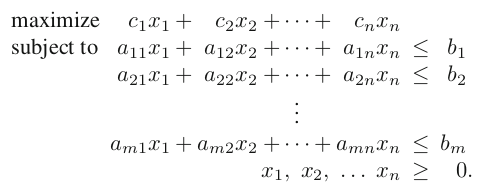
\includegraphics[width=.9\linewidth]{Introduction (1)/screenshot_2019-01-28_08-20-31.png}
\end{center}
\begin{itemize}
\item Linear programs formulated this way is refereed to as linear programs in standard form
\begin{itemize}
\item \(m\) is used to denote the number of constrains
\item \(n\) is used to denote the number of decision variables
\end{itemize}

\item A proposal of specific values for the decision variables is called a \textbf{solution}
\item A solution \((x_1, x_2, \dots, x_n)\) is called \textbf{feasible} if it satisfies all of the constraints
\begin{itemize}
\item It is called \textbf{optimal} if it also attains the desired maximum
\item Problems are \textbf{infeasible} when there exists no feasible solution
\item Problems is \textbf{unbounded} if it has feasible solution with arbitrarily large objective values
\end{itemize}
\end{itemize}

\section{The Simplex Method}
\label{sec:org5812b7f}
\subsection{Problem}
\label{sec:org7311ee7}
\begin{itemize}
\item Given a general linear programming problem presented in standard form:
\end{itemize}
\begin{center}
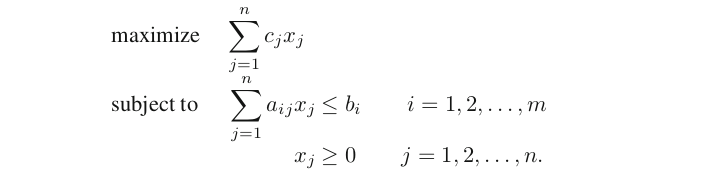
\includegraphics[width=.9\linewidth]{The Simplex Method/screenshot_2019-01-28_08-52-51.png}
\end{center}

\begin{itemize}
\item The first task is to introduce slack variables and a name for the objective function value
\end{itemize}
\begin{center}
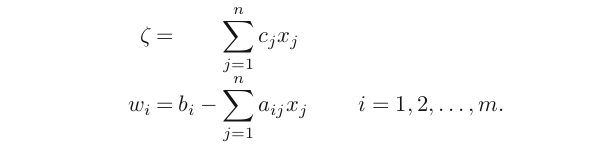
\includegraphics[width=.9\linewidth]{The Simplex Method/screenshot_2019-01-28_08-53-05.png}
\end{center} 

\subsection{Basic and nonbasic variables}
\label{sec:org04f6f90}
\begin{itemize}
\item The list of slack variables are added to the list of \(x\) variables
\end{itemize}
\begin{equation}
  (x_1, \dots, x_n, w_1, \dots, w_m) = (x_1, \dots, x_n, x_{n+1}, \dots, x_{n+m})
\end{equation}
\begin{itemize}
\item With this notation the problem can be rewritten as
\end{itemize}
\begin{center}
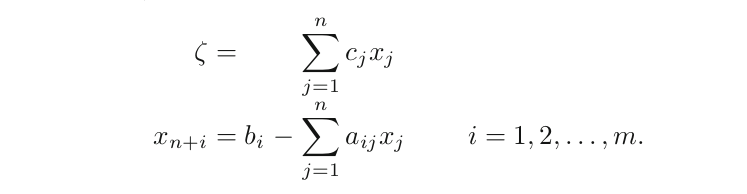
\includegraphics[width=.9\linewidth]{The Simplex Method/screenshot_2019-01-28_08-58-57.png}
\end{center}  

\begin{itemize}
\item This is the \textbf{starting dictionary}
\item As the simplex method progresses it moves from one dictionary to another in search for an optimal solution
\begin{itemize}
\item As dictionary has \(m\) basic variables and \(n\) nonbasic variables
\item Let \(\mathcal B\) denote the collection of indices from \(\{1,2,\dots, n+m\}\) corresponding to the basic variables
\begin{itemize}
\item Initially \(\mathcal N = \{n+1, n+2, \dots, n+m\}\)
\end{itemize}
\item Let \(\mathcal N\) denote the indices corresponding to the nonbasic variables
\begin{itemize}
\item Initially \(\mathcal B = \{1,2, \dots, n\}\)
\end{itemize}
\item In an iteration the current dictionary will look like this
\end{itemize}
\end{itemize}
\begin{center}

\includegraphics[width=.9\linewidth]{The Simplex Method/screenshot_2019-01-28_09-15-11.png}
\end{center}

\subsection{Choosing the variables}
\label{sec:orgfc8dd7e}
\begin{itemize}
\item In each iteration of the simplex method exactly one variable goes from nonbasic to basic and exactly one goes from basic to nonbasic
\begin{itemize}
\item The variable that goes from nonbasic to basic is called the \textbf{entering variable}
\begin{itemize}
\item It is chosen with the aim of increasing \(\zeta\)
\item One whose coefficient is positive
\item Pick \(k\) from \(\{j \in \mathcal N \mid \bar c_j > 0 \}\)
\begin{itemize}
\item If the set is empty the current solution is optimal
\end{itemize}
\item The \(k\) that is usually picked is the one with the largest coefficient
\end{itemize}
\item The variable that goes from basic to nonbasic is called the \textbf{leaving variable}
\begin{itemize}
\item It is chosen to preserve non-negativity of the current basic variables
\item Once we have decided that \(x_k\) will be the entering variable its value will be increased from 0 to a positive value
\begin{itemize}
\item The increase will change the values of the basic variables: \(x_i = \bar b_i - \bar a_{ik}x_k \quad i \in \mathcal B\)
\end{itemize}
\item To ensure that each of the variables remains nonnegative we must require that
\begin{itemize}
\item \(\bar b_i - \bar a_{ik} x_k \geq 0 \quad i \in \mathcal B\)
\end{itemize}
\item Since the only ones that can go negative as \(x_k\) increases are those for which \(\bar a_{ik}\) is positive
\begin{itemize}
\item The value \(x_k\) at which the expression becomes zero is \(x_k = \bar b_i / \bar a_{ik}\)
\item \(x_k\) can only be raised to the smallest of these values \(x_k = \min_{i \in \mathcal B : \hat a_{ik} > 0} \hat b_i / \hat a_{ik}\)
\end{itemize}
\item The rule for selecting the leaving variable is pick \(l\) from \(\{i \in \mathcal B \mid \hat a_{ik} > 0 \text{ and } \hat b_i / \hat a_{ik} \text{ is minimal }\}\)
\end{itemize}
\end{itemize}

\item Once the leaving-basic and entering basic variables have been selected the move from the current dictionary to a new dictionary involves appropriate row operations
\begin{itemize}
\item This step is called a \textbf{pivot}
\end{itemize}
\item Rules that make the choice of leaving variables unambiguous are called \textbf{pivot rules}
\end{itemize}

\subsection{Initialization}
\label{sec:org6ad8b86}
\begin{itemize}
\item The solution associated with the initial dictionary is obtained by setting each \(x_j\) to zero and setting each \(w_i\) equal to the corresponding \(b_i\)
\begin{itemize}
\item This solution is only feasible if and only if all the right-hand sides are nonnegative
\end{itemize}

\item If the right hand side is not nonnegative and auxiliary problem is defined for which 
\begin{enumerate}
\item A feasible dictionary is easy to find
\item The optimal dictionary provides a feasible dictionary for the original problem
\end{enumerate}

\item The auxiliary problem is
\end{itemize}
\begin{center}
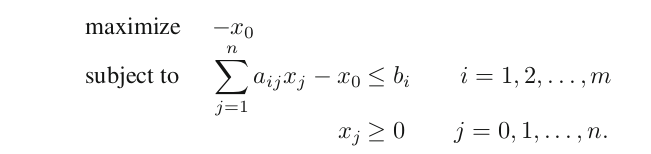
\includegraphics[width=.9\linewidth]{The Simplex Method/screenshot_2019-01-28_09-59-24.png}
\end{center}
\begin{itemize}
\item It is easy to give a feasible solution to the auxilary problem
\begin{itemize}
\item Simply set \(x_j = 0\) for \(j=1, \dots, n\) and then pick \(x_0\) to be sufficiently large
\item Often referred to as \textbf{Phase I}
\end{itemize}
\end{itemize}

\subsection{Unboundedness}
\label{sec:orgc2a507c}
\begin{itemize}
\item If none of the ratios are positive the problem is unbounded
\end{itemize}

\section{Degeneracy}
\label{sec:org1a17b73}
\subsection{Definition}
\label{sec:org0876cc9}
\begin{itemize}
\item A dictionary is \textbf{degenerate} if \(\bar b_i\) vanishes for some \(i \in \mathcal B\)
\begin{itemize}
\item A degenerate dictionary could cause difficulties for the simplex algorithm but it might not
\item Problems arise when a degenerate dictionary produces degenerate pivots
\begin{itemize}
\item A pivot is degenerate is the calculation of the leaving variable is \(+ \infty\)
\item If the numerate is positive and the denominator vanishes
\end{itemize}
\item If might happen that the simplex algorithm will make a sequence of degenerate pivots and eventually return to a dictionary that has appeared before
\begin{itemize}
\item This is called \textbf{cycling}
\item It is typical for a pivot to "break away" from the degeneracy
\end{itemize}
\item Under certain pivoting rules cycling is possible this could e.g. be 
\begin{itemize}
\item Choose the entering variable as the one with the largest coefficient in the \(\varsigma\) row of the dictionary
\item When two or more variables compete for leaving the basis, pick an \(x\) variable over a slack variable
\begin{itemize}
\item If there is a choice use the variable with the smallest subscript
\item This means reading left to right, pick the first leaving candidate from the list: \(x_1,x_2, \dots, x_n, w_1, w_2, \dots, w_m\)
\end{itemize}
\item It is hard to find examples of cycling in which \(m\) and \(n\) are small
\begin{itemize}
\item It has been shown that if a problem has an optimal solution but cycles off-optimum the problem must involve dictionary with at least four non-slack variables and two constraints
\end{itemize}
\end{itemize}
\end{itemize}

\item \textbf{Theorem 3.1.} If the simplex method fails to terminate, then it must cycle
\begin{itemize}
\item \textbf{Proof intuition:} there is a finite amount of dictionaries if it does not terminate it must cycle
\end{itemize}
\end{itemize}

\subsection{The Perturbation/Lexicographic Method}
\label{sec:orgf21393c}
\begin{itemize}
\item The simplex method is a whole family of related algorithms from which we can pick a specific instance by specifying what we have been referring to as pivoting rules
\item There are pivoting rules for the simplex algorithm in which one either reach an optimal solution or prove that no such solution exists
\item One of the methods is based on the observation that degeneracy is sort of an accident
\begin{itemize}
\item A dictionary is degenerate if one or more of the \(\bar b_i\) vanish
\item The right hand side could be any real number
\begin{itemize}
\item The probability of the occurrence of any specific number is quite unlikely
\item Permute the problem by adding small random perturbation independently
\begin{itemize}
\item The probability of exact cancellation is zero if they are chosen independently
\end{itemize}
\end{itemize}
\item Small positive numbers \(\epsilon_1, \dots, \epsilon_m\) are introduced for each constraint where the perturbation is getting much smaller on each succeeding constraint
\begin{itemize}
\item It is written as \$0<\(\epsilon_{\text{m}}\) << \dots{} << \(\epsilon_{\text{2}}\) << \(\epsilon_{\text{1}}\) << \$ all other data
\item The idea is that each \(\epsilon_i\) acts on an entirely different scale from all the other \(\epsilon_i\)'s
\begin{itemize}
\item No linear combination of the \(\epsilon_i\) using coefficients that might arise will ever produce a number whose size is the same scale as the data in the problem
\item Instead of using specific values they are simply treat them as abstract symbols having these scale properties which is called the lexicographic method
\end{itemize}
\end{itemize}
\end{itemize}

\item \textbf{Theorem} The simplex method always terminates provided that the leaving variable is selected by the lexicographic rule
\end{itemize}

\subsection{Bland's Rule}
\label{sec:org651d082}
\begin{itemize}
\item Bland's rule stipulates that both the entering and the leaving variable be elected from their respective sets of choices by choosing the variable \(x_k\) with the smallest index \(k\)
\item \textbf{Theorem} The simplex method always terminates provided that both the entering and leaving variable are chosen according to Bland's rule
\end{itemize}

\subsection{Fundamental Theorem of Linear Programming}
\label{sec:org9198de7}
\begin{itemize}
\item \textbf{Theorem} For an arbitrary linear program in standard form the following statements are true
\begin{enumerate}
\item If there is no optimal solution, then the problem is either infeasible or unbounded
\item If a feasible solution exists, then a basic feasible solution exists
\item If an optimal solution exists then a basic optimal solution exists
\end{enumerate}
\end{itemize}

\section{Efficiency of the Simplex Method}
\label{sec:org24d1e6b}
\subsection{Worst-Case Analysis}
\label{sec:org07ec894}
\begin{itemize}
\item For noncycling variants of the simplex method the simplex method moves from one basic feasible solution to another
\begin{itemize}
\item This is without returning to a previously visited solution
\item The upper bound for the number iterations is simply the number of basic feasible solution which there can be at most \(\binom{n+m}{m}\)
\item The bound is maximized when \(n=m\)
\begin{itemize}
\item It is bounded by \(2^{2n}\)
\item This is very huge even when \(n\) is very small
\end{itemize}
\end{itemize}

\item The following is a linear problem proposed in 1972 by V.Klee and G.J. Minty which requires \(2^n-1\) iterations to solve
\end{itemize}
\begin{center}
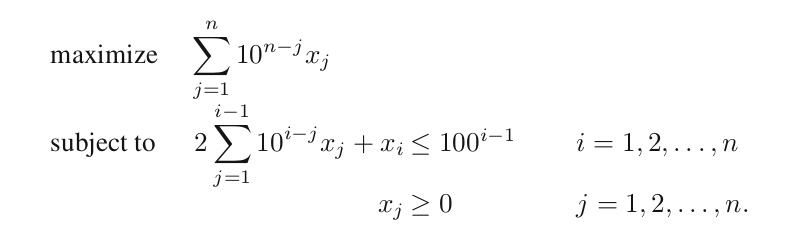
\includegraphics[width=.9\linewidth]{Efficiency of the Simplex Method/screenshot_2019-02-06_10-28-46.png}
\end{center}
\begin{itemize}
\item The simplex method with the largest coefficient rule will start at one of these vertices and visit every vertex before finding the optimal solution
\begin{itemize}
\item The idea is that the RHS of the conditions have the following conditions
\end{itemize}
\end{itemize}
\begin{equation}
 1 = b_1 << b2 << \cdots << b_n 
\end{equation}
\begin{itemize}
\item No one has found a rule that is better than the largest coefficient rule for Simplex
\end{itemize}

\subsection{Empirical Average Performance of the Simplex Method}
\label{sec:orgb07498a}
\begin{itemize}
\item The best measure is \(min(n,m)\)
\end{itemize}

\section{Duality Theory}
\label{sec:orge9edd23}
\subsection{The Dual Problem}
\label{sec:org7a714ba}
\begin{itemize}
\item Given a linear programming problem in standard form, which is called the \textbf{primal problem}
\end{itemize}
\begin{center}
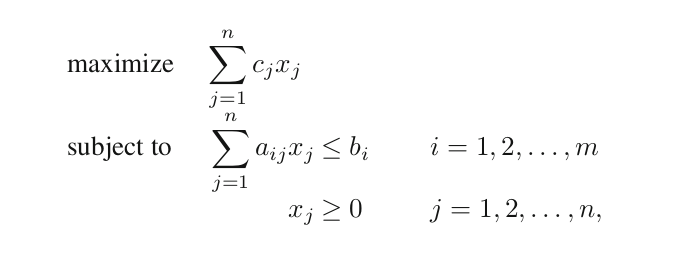
\includegraphics[width=.9\linewidth]{Duality Theory/screenshot_2019-02-06_11-01-43.png}
\end{center}
\begin{itemize}
\item the associated \textbf{dual linear program} is given by
\begin{center}
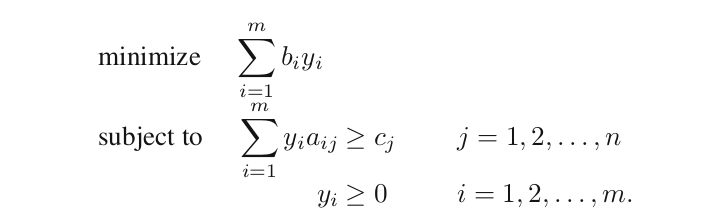
\includegraphics[width=.9\linewidth]{Duality Theory/screenshot_2019-02-06_11-02-30.png}
\end{center}

\item Taking the dual of the dual returns us to the primal
\item The dual problem provides upper bounds for the primal objective function value
\end{itemize}

\subsection{The Weak Duality Theorem}
\label{sec:org97cb2fa}
\begin{itemize}
\item \textbf{Theorem} If \((x_1, x_2, \dots, x_n)\) is feasible for the primal and \((y_1, y_2, \dots, y_n)\) is feasible for the dual then
\end{itemize}
\begin{equation}
  \sum_j c_jx_j \leq \sum_i b_iy_i 
\end{equation}

\subsection{The Strong Duality Theorem}
\label{sec:org9e85167}
\begin{center}
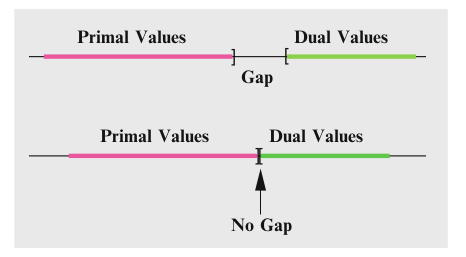
\includegraphics[width=.9\linewidth]{Duality Theory/screenshot_2019-02-06_11-12-19.png}
\end{center} 

\begin{itemize}
\item \textbf{Theorem} If the primal problem has an optimal solution
\end{itemize}
\begin{equation}
  x^*= (x_1^*, x_2^*, \dots, x_n^*)
\end{equation}	
\begin{itemize}
\item then the dual has an optimal solution
\end{itemize}
\begin{equation}
  y^*= (y_1^*, y_2^*, \dots, y_n^*)
\end{equation}	
such that	
\begin{equation}
  \sum_j c_j x_j^* = \sum_i b_i y_i^*
\end{equation}	

\begin{itemize}
\item If the primal problem is unbounded the dual problem is infeasible
\begin{itemize}
\item If the dual problem is unbounded then the primal problem must be infeasible
\end{itemize}

\item Duality theory provides a certificate of optimality
\begin{itemize}
\item One can check that the two given solutions for the dual and primal problem is feasible
\item One can check that the two solutions are equal
\end{itemize}

\item Sometimes it is easy to apply the simplex method to the dual
\end{itemize}

\subsection{Complementary Slackness}
\label{sec:org62afd89}
\begin{itemize}
\item \textbf{Theorem} Suppose that \(x=(x_1,x_2,\dots,x_n)\) is primal feasible and \(y=(y_1,y_2,\dots,y_m)\) is dual feasible. Let \((w_1, w_2, \dots, \dots, w_m)\) denote the corresponding primal slack variable and let \((z_1, z_2, \dots, z_n)\) denote the corresponding dual slack variable. Then \(x\) and \(y\) are optimal for the respective problems if and only if
\end{itemize}
\begin{align}
  x_jz_h &= 0, \quad \text{for } j=1, 2, \dots,n \\
  w_iy_i &= 0, \quad \text{for } i=1, 2, \dots,n
\end{align}
\begin{itemize}
\item This can be used to find the solution to the corresponding dual problem given an optimal feasible solution to the primal problem
\end{itemize}

\subsection{The Dual Simplex Method}
\label{sec:org0821a3a}
\begin{itemize}
\item By using the simplex algorithm on the dual problem while keeping track of corresponding primal, this can be used to find feasible dictionary for the primal problem
\begin{itemize}
\item This is done if the starting dictionary for the dual problem is feasible but the one for the primal is not
\end{itemize}
\end{itemize}

\subsection{A Dual-Based Phase I Algorithm}
\label{sec:orgd1e38cf}
\begin{itemize}
\item If both the starting dictionary for the dual and primal problem are infeasible one can change the primal problem to make the corresponding dual problem feasible
\begin{itemize}
\item This can finding a feasible starting dictionary for the primal problem
\end{itemize}
\end{itemize}

\subsection{The Dual of a Problem in General Form}
\label{sec:org4fe6723}
\begin{center}
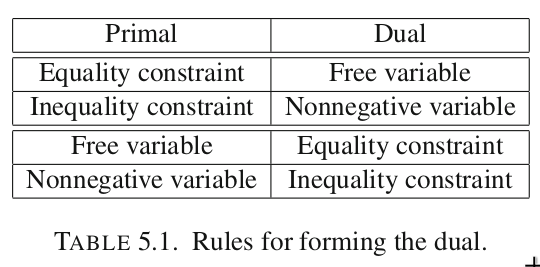
\includegraphics[width=.9\linewidth]{Duality Theory/screenshot_2019-02-06_11-47-39.png}
\end{center}
\begin{itemize}
\item Free variables are unconstrained variables

\item Given the following linear programming problem
\end{itemize}
\begin{center}
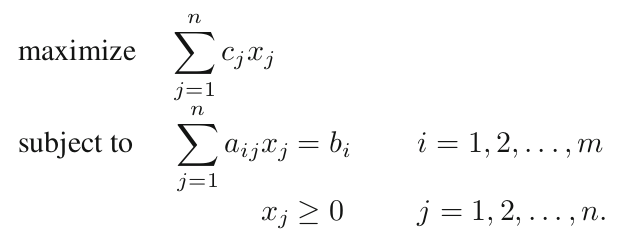
\includegraphics[width=.9\linewidth]{Duality Theory/screenshot_2019-02-06_11-49-18.png}
\end{center}
\begin{itemize}
\item The corresponding dual is
\end{itemize}
\begin{center}
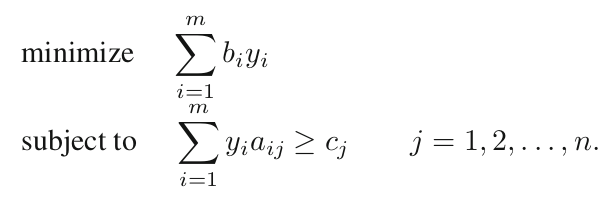
\includegraphics[width=.9\linewidth]{Duality Theory/screenshot_2019-02-06_11-49-53.png}
\end{center}

\section{Convex Analysis}
\label{sec:orgabb7627}
\subsection{Farkas' Lemma}
\label{sec:org333a99f}
\begin{itemize}
\item The system \(Ax \leq b\) has no solutions if and only if there is a \(y\) such that
\end{itemize}
\begin{align*}
  A^T y &= 0\\ 
  y &\geq 0\\ 
  b^T y &< 0
\end{align*}

\subsection{Strict Complementarity}
\label{sec:org14b2d9b}
\begin{itemize}
\item \textbf{Theorem} If both the primal and the dual have feasible solutions, then there exists a primal feasible solution \((\bar x, \bar w)\) and a feasible solution \((\bar y, \bar z)\) such that \(\bar x + \bar z > 0\) and \((\bar y + \bar w) > 0\)
\item A variable \(x_j\) that must vanish in order for a linear programming problem to be feasible is called a \textbf{null variable}
\item \textbf{Strict Complementarity Slackness Theorem:} If a linear programming problem has an optimal solution, then there is an optimal solution \((x^*, w^*)\) and an optimal dual solution \((y^*,z^*)\) such that \(x^* + z^* > 0\) and \(y^* + w^* > 0\)
\end{itemize}
\section{Game Theory}
\label{sec:orgddc61b8}
\subsection{Matrix Games}
\label{sec:orgd46840e}
\begin{itemize}
\item A \textbf{matrix game} is a two person game which is defined as follows
\begin{itemize}
\item First each person selects an action from a finite set of choices 
\begin{itemize}
\item Done independently of the other
\item They will in general be confronted with different set of actions
\end{itemize}
\item Then Both reveal to each other their choice
\begin{itemize}
\item \(i\) denote the first player's choice
\item \(j\) denote the second player's choice
\item The rules of the game stipulate that the first player will pay the second player \(a_{ij}\) dollars
\end{itemize}
\item The array of possible payments \(A = [a_{ij}]\) is presumed to be known to both players before the game begins
\begin{itemize}
\item If the payment is negative for some \((i,j)\) the payment goes in the other direction
\end{itemize}
\item The first player is refereed to as the \textbf{row player} and the second as \textbf{column player}
\item Since the is a finite number of actions for each player \(i\) is a number selected from \(1\) to \(m\) and \(j\) is selected from \(1\) to \(n\)
\item Rock paper scissors can be described as a matrix game in the following way
\end{itemize}
\end{itemize}
\begin{equation}
  \begin{bmatrix} 
     0 &  1 & -1 \\ 
    -1 &  0 &  1 \\ 
     1 & -1 &  0 
  \end{bmatrix}
\end{equation}	

\begin{itemize}
\item \textbf{Randomized strategy} means that each play of the game appears from the other players point of view that the player is making the choices random according to some probability distribution
\begin{itemize}
\item Let \(y_i\) denote the probability that the row player selects action \(i\)
\begin{itemize}
\item The vector \(y\) composed of these probabilities is called a \textbf{stochastic vector}
\end{itemize}
\item Mathematically a vector is a stochastic vector if it has nonnegative components that sum to one
\begin{itemize}
\item i.e. \(y \geq 0\)  and \(e^T y = 1\) where \(e\) is a vector consisting of all ones
\end{itemize}
\item The column players must also adopt a randomized strategy
\item Let \(x_j\) denote the probability that the column player selects action \(j\)
\begin{itemize}
\item Let \(x\) denote the stochastic vector composed of these probabilities
\end{itemize}
\item The expected payoff of the column player is computed by summing over all possible outcomes
\begin{itemize}
\item The payoff associated becomes the outcome times the probability of that outcome
\end{itemize}
\item The set of the possible outcomes is simply the set of pairs \((i,j)\)
\begin{itemize}
\item \(i\) ranges over the row indices \((1,2,\dots,m)\)
\item \(j\) ranges over the column indices \((1,2,\dots,n)\)
\end{itemize}
\item The expected payoff to the column players is
\end{itemize}
\end{itemize}
\begin{equation*}
  \sum_{i,j} y_ia_{ij}x_j = y^T A x
\end{equation*}

\subsection{Optimal Strategies}
\label{sec:org11a773e}
\begin{itemize}
\item If the column player adopts strategy \(x\) the row player's then the row player's best defense is to use the strategy \(y^*\) that achieves the following minimum
\end{itemize}

\begin{center}

\includegraphics[width=.9\linewidth]{Game Theory/screenshot_2019-02-11_15-09-18.png}
\end{center}

\begin{itemize}
\item Since for any given \(x\) the row player will adopt the strategy that achieves the minimum in the previous problem the column player should employ a strategy \(x^*\) that attains the following maximum
\end{itemize}
\begin{equation*}
  \max_x \ \min_y \ y^T A x
\end{equation*}
\begin{itemize}
\item where max and the min are over all stochastic vectors 
\begin{itemize}
\item This problem can be reformulated as a linear programming problem
\item The inner optimization can be taken over just the deterministic strategies
\end{itemize}
\end{itemize}
\begin{equation}
  \min_y y^T Ax = \min_i e_i^T Ax
\end{equation}
\begin{itemize}
\item The max-min problem can be rewritten as
\end{itemize}
\begin{center}
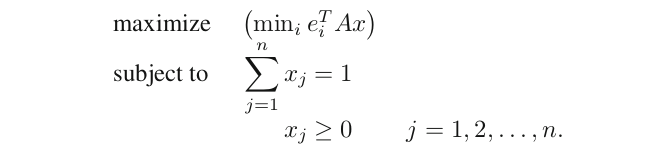
\includegraphics[width=.9\linewidth]{Game Theory/screenshot_2019-02-11_15-22-34.png}
\end{center}
\begin{itemize}
\item If one introduce a new variable \(v\) representing a lower bound on the \(e_i^TAx\) the problem can be recast as a linear program
\end{itemize}
\begin{center}
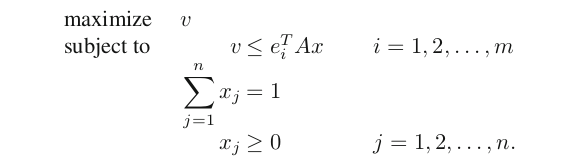
\includegraphics[width=.9\linewidth]{Game Theory/screenshot_2019-02-11_15-25-15.png}
\end{center} 
\begin{itemize}
\item In vector notation it is written as
\end{itemize}
\begin{center}

\includegraphics[width=.9\linewidth]{Game Theory/screenshot_2019-02-11_15-25-41.png}
\end{center}
\begin{itemize}
\item In block-matrix form one gets
\end{itemize}
\begin{center}
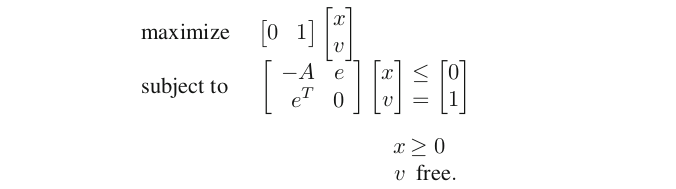
\includegraphics[width=.9\linewidth]{Game Theory/screenshot_2019-02-11_15-26-42.png}
\end{center}

\begin{itemize}
\item By symmetry the row player seeks a strategy \(y^*\) that attains optimality in the following min-max problem:
\end{itemize}
\begin{equation*}
  \min_y \ \max_x y^TAx
\end{equation*}
\begin{itemize}
\item which can be reformulated as the linear program
\end{itemize}
\begin{center}

\includegraphics[width=.9\linewidth]{Game Theory/screenshot_2019-02-11_15-28-56.png}
\end{center}
\begin{itemize}
\item Written in block-matrix form we get
\end{itemize}
\begin{center}
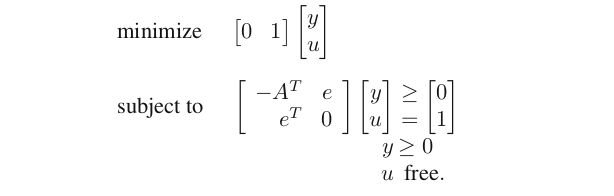
\includegraphics[width=.9\linewidth]{Game Theory/screenshot_2019-02-11_15-29-44.png}
\end{center} 

\subsection{The Minimax Theorem}
\label{sec:org94e0777}
\begin{itemize}
\item \textbf{Minimax Theorem} There exist stochastic vectors \(x^*\) and \(y^*\) for which
\end{itemize}
\begin{equation}
  \max_x y^{* ^T} Ax = \min_y y^T A x^*
\end{equation}
\begin{itemize}
\item Proof using the strong duality theorem

\item The common optimal value \(v^* = u^*\) is called the \textbf{value} of the game
\begin{itemize}
\item A game whose value is zero is a fair game
\item Games where the two players are interchangeable are fair
\begin{itemize}
\item They are called \textbf{symmetric}
\item They are characterized by payoff matrices having the property that \(a_{ij} = -a_{ji}\) for all \(i\) and \(j\)
\end{itemize}
\end{itemize}
\end{itemize}

\section{The Simplex Method in Matrix Notation}
\label{sec:org845ae6c}
\subsection{Matrix Notation}
\label{sec:orgaf37900}
\begin{itemize}
\item A standard-form linear programming problem
\begin{center}
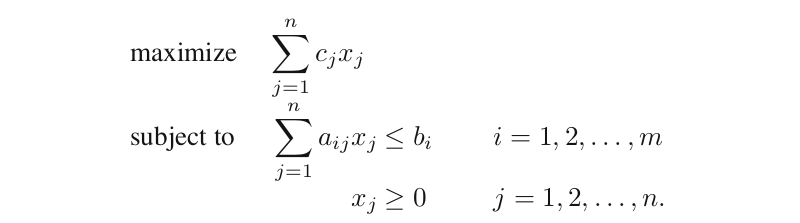
\includegraphics[width=.9\linewidth]{The Simplex Method in Matrix Notation/screenshot_2019-02-11_15-56-17.png}
\end{center}
\item It the be written in matrix for the following way with the slack variables denoted as \(x_{n+i}\) instead of \(w_i\)  
\begin{center}

\includegraphics[width=.9\linewidth]{The Simplex Method in Matrix Notation/screenshot_2019-02-11_15-57-54.png}
\end{center}
\item where
\end{itemize}
\begin{center}
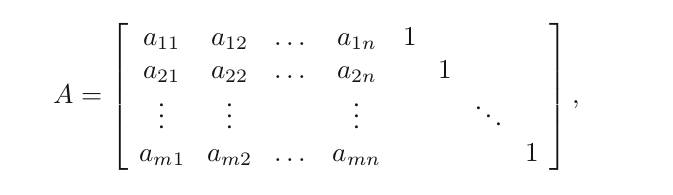
\includegraphics[width=.9\linewidth]{The Simplex Method in Matrix Notation/screenshot_2019-02-11_15-58-09.png}
\end{center}
\begin{itemize}
\item and
\end{itemize}
\begin{center}
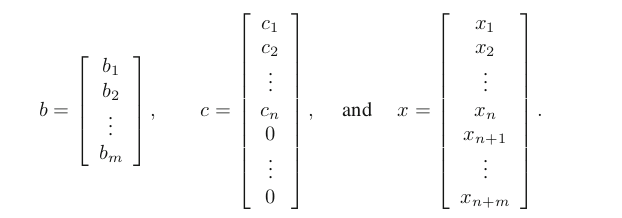
\includegraphics[width=.9\linewidth]{The Simplex Method in Matrix Notation/screenshot_2019-02-11_15-59-28.png}
\end{center}
\begin{itemize}
\item In component notation the \$i\$th component of \(Ax\) can be broken up into a basic part and a nonbasic part
\end{itemize}
\begin{equation}
  \sum_{j=1}^{n+m}a_{ij}x_j = \sum_{j \in \mathcal B} x_j + \sum_{j \in \mathcal N} x_j 
\end{equation}	
\begin{itemize}
\item We let \(B\) denote an \(m \times m\) matrix whose columns consists precisely of the \(m\) columns of \(A\) that are associated with the basic variables
\begin{itemize}
\item \(N\) denote an \(m \times n\) matrix whose columns are the \(n\) nonbasic columns of \(A\)
\item \(A\) is written in an partitioned matrix form as follows \(A= [B \quad N]\)
\begin{itemize}
\item The matrix on the right does not equal the \(A\) matrix
\item It is the \(A\) matrix with its columns rearranged in such a manner that all the columns associated with basic variables are listed first followed by the nonbasic
\end{itemize}
\item Let rearrange the rows of \(x\) and write
\end{itemize}
\end{itemize}
\begin{equation}
	x = 
	\begin{bmatrix}
		x_{\mathcal B} \\ x_{\mathcal N}
	\end{bmatrix}
\end{equation}
\begin{itemize}
\item Then the following separation of \(Ax\) into a sum of two terms is true and captures the separation of variables
\end{itemize}
\begin{equation}
  Ax = [B \quad N]
	\begin{bmatrix}
		x_{\mathcal B} \\ x_{\mathcal N}
	\end{bmatrix}
	= B x_{\mathcal B} + N x_{\mathcal N}
\end{equation}
\begin{itemize}
\item By similarly partitioning \(c\) one can write
\end{itemize}
\begin{center}
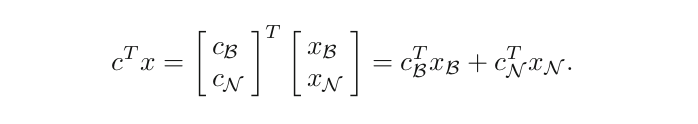
\includegraphics[width=.9\linewidth]{The Simplex Method in Matrix Notation/screenshot_2019-02-11_16-13-39.png}
\end{center}

\subsection{The Primal Simplex Method}
\label{sec:org2f54449}
\begin{itemize}
\item A dictionary has the property that the basic variables are written as functions of the nonbasic variables
\begin{itemize}
\item The constrain equations \(Ax = b\) can be written as \(B x_{\mathcal B} + N x_{\mathcal N} = b\)
\item The fact that basic variables \(x_{\mathcal B}\) can be written as a function of the nonbasic variables is equivalent to the fact that the matrix \(B\) is invertible and therefore
\end{itemize}
\end{itemize}
\begin{center}

\includegraphics[width=.9\linewidth]{The Simplex Method in Matrix Notation/screenshot_2019-02-11_16-26-40.png}
\end{center}
\begin{itemize}
\item The objective function can be written as
\end{itemize}
\begin{center}
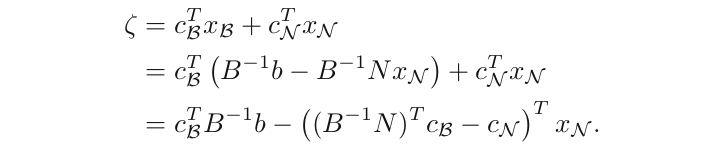
\includegraphics[width=.9\linewidth]{The Simplex Method in Matrix Notation/screenshot_2019-02-11_16-27-18.png}
\end{center}
\begin{itemize}
\item The dictionary associated with basic \(\mathcal B\) can be written as
\end{itemize}
\begin{center}

\includegraphics[width=.9\linewidth]{The Simplex Method in Matrix Notation/screenshot_2019-02-11_16-28-16.png}
\end{center}
\begin{itemize}
\item Based on the component-form notation the following identifications can be made
\end{itemize}
\begin{center}
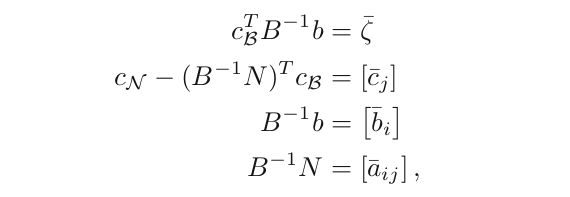
\includegraphics[width=.9\linewidth]{The Simplex Method in Matrix Notation/screenshot_2019-02-11_16-29-26.png}
\end{center}
\begin{itemize}
\item where the bracketed expressions on the right denote vectors and matrices with the index \(i\) running over \(\mathcal B\) and the index \(j\) running over \(\mathcal N\)
\item The basic solution associated with the dictionary is obtained by settings \(x_{\mathcal N}\) equal to zero
\end{itemize}
o\begin{center}

\includegraphics[width=.9\linewidth]{The Simplex Method in Matrix Notation/screenshot_2019-02-11_16-33-51.png}
\end{center}

\begin{itemize}
\item For the dual slack variables we need to relabel the dual variables and append them to the dual slacks such that \(y_i\) becomes \(z_{n+i}\)
\begin{itemize}
\item Using the relabeling of the dual variables the dual dictionary corresponding to a given primal dictionary is
\end{itemize}
\end{itemize}
\begin{center}
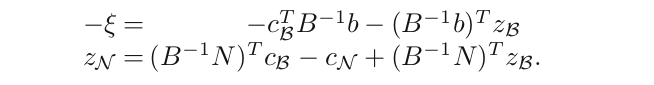
\includegraphics[width=.9\linewidth]{The Simplex Method in Matrix Notation/screenshot_2019-02-11_16-40-08.png}
\end{center} 
\begin{itemize}
\item The dual solution associated with this dictionary is obtained by setting \(z_{\mathcal B}\) equal to zero
\end{itemize}
\begin{center}

\includegraphics[width=.9\linewidth]{The Simplex Method in Matrix Notation/screenshot_2019-02-11_16-40-59.png}
\end{center} 
\begin{itemize}
\item The following shorthand can be introduced
\end{itemize}
\begin{center}

\includegraphics[width=.9\linewidth]{The Simplex Method in Matrix Notation/screenshot_2019-02-11_16-44-45.png}
\end{center}
\begin{itemize}
\item The primal dictionary can be written succinctly as
\end{itemize}
\begin{center}
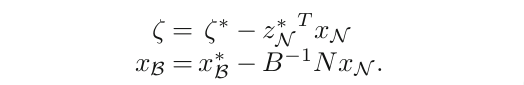
\includegraphics[width=.9\linewidth]{The Simplex Method in Matrix Notation/screenshot_2019-02-11_16-45-20.png}
\end{center}
\begin{itemize}
\item The associated dual dictionary has a very symmetric appearance
\end{itemize}
\begin{center}

\includegraphics[width=.9\linewidth]{The Simplex Method in Matrix Notation/screenshot_2019-02-11_16-49-40.png}
\end{center}

\begin{itemize}
\item The primal simplex method can be described as follows.
\begin{itemize}
\item The starting assumptions are that we are given
\begin{enumerate}
\item A partition of the \(n+m\) indices into a collection \(\mathcal B\) of \(m\) basic indices and a collection \(\mathcal N\) of \(n\) nonbasic ones with the property that the basic matrix \(B\) is invertible
\item An associated current primal solution \(x_{\mathcal B}^* \geq 0\) (and \(x_{\mathcal N}^* = 0\))
\item An Associated current dual solution \(z_{\mathcal N}^*\) (with \(z_{\mathcal B} = 0\))
\end{enumerate}
\item The simplex algorithm then produces a sequence of steps to "adjacent" bases such that the current value \(\varsigma^*\) of the objective function \(\varsigma\) increases at each step updating \(x_{\mathcal B}^*\) and \(x_{\mathcal N}^*\) along the way
\begin{itemize}
\item If the step size is positive
\end{itemize}
\item Two bases are said to be adjacent to each other if they differ in only one index
\begin{itemize}
\item i.e. given a basic \(\mathcal B\) an adjacent basic is determined by removing one basic index and replacing it with a nonbasic index
\item The index that gets removed corresponds to the leaving variable
\end{itemize}
\item One step of the simplex method is called an iteration
\item An iteration runs as follows
\begin{enumerate}
\item \textbf{Check for optimality}
\begin{itemize}
\item If \(z ^* _{\mathcal N} \geq 0\) stop. The current situation is optimal
\item All that is required for optimality is dual feasibility and that is the case if an only if \(z ^*_{\mathcal N} \geq 0\)
\end{itemize}
\item \textbf{Select Entering Variable}
\begin{itemize}
\item Pick an index \(j \in \mathcal N\) for which \(z_j^* < 0\)
\item Variable \(x_j\) is the entering variable
\end{itemize}
\item \textbf{Compute Primal Step Direction} \(\Delta x_\mathcal B\)
\begin{itemize}
\item Having selected the entering variable we want to increase its value from zero and we let \(x_{\mathcal N} = t e_j\)
\item Then we have that from the primal dictionary that \(x_{\mathcal B} = x^*_{\mathcal B} - B^{-1} N t e_j\)
\item The step direction \(\Delta x_{\mathcal B}\) is given by \(\Delta x_{\mathcal B} = B^{-1} N e_j\)
\end{itemize}
\item \textbf{Compute Primal Step Length}
\begin{itemize}
\item We want to pick the largest \(t \geq 0\) for which every component of \(x_{\mathcal B}\) remains nonnegative
\begin{itemize}
\item i.e. we want to pick the largest \(t\) for which \(x^*_{\mathcal B} \geq t \Delta x_{\mathcal B}\)
\end{itemize}
\item The largest \(t\) for which all of the inequalities hold is given by \(t = \big(\max_{i \in \mathcal B} \frac{\Delta x_i}{x_i^*}\big)^{-1}\)
\begin{itemize}
\item The correct convention for \(0/0\) is to set such ratios equal to zero
\item If the maximum is less than or equal to zero we can stop here the primal is unbounded
\end{itemize}
\end{itemize}
\item \textbf{Select Leaving Variable}
\begin{itemize}
\item The leaving variable is chosen as any variable \(x_i, i \in \mathcal N\) for which the maximum in the calculation of \(t\) is obtained
\end{itemize}
\item \textbf{Compute Dual Step Direction} \(\Delta z_{\mathcal N}\)
\begin{itemize}
\item Since in that dictionary \(z_i\) is the entering variable we see that
\begin{itemize}
\item \(\Delta z_{\mathcal N} = -(B^{-1} N) ^T e_i\)
\end{itemize}
\end{itemize}
\item \textbf{Compute Dual Step Length}
\begin{itemize}
\item Since we known that \(z_j\) is the leaving variable in the dual dictionary the step length for the dual variables is
\begin{itemize}
\item \(s = \frac{z_j^*}{\Delta z_j}\)
\end{itemize}
\end{itemize}
\item \textbf{Update Current Primal and Dual solutions}
\begin{itemize}
\item Now everything has been obtained to update the data in the dictionary
\begin{itemize}
\item \(x_j^* \leftarrow t\)
\item \(x_{\mathcal B}^* \leftarrow x_{\mathcal B}^* - t \Delta x_{\mathcal B}\)
\end{itemize}
\item and
\begin{itemize}
\item \(z_i^* \leftarrow s\)
\item \(z_{\mathcal N}^* \leftarrow z_{\mathcal N}^* - s \Delta z_{\mathcal N}\)
\end{itemize}
\end{itemize}
\item \textbf{Update Basis}
\begin{itemize}
\item The basis is updated \(\mathcal B \leftarrow \matchcal B \backslash \{ i \} \cup \{ j \}\)
\end{itemize}
\end{enumerate}
\end{itemize}
\end{itemize}

\subsection{The Dual Simplex Method}
\label{sec:org586cd05}
\begin{center}
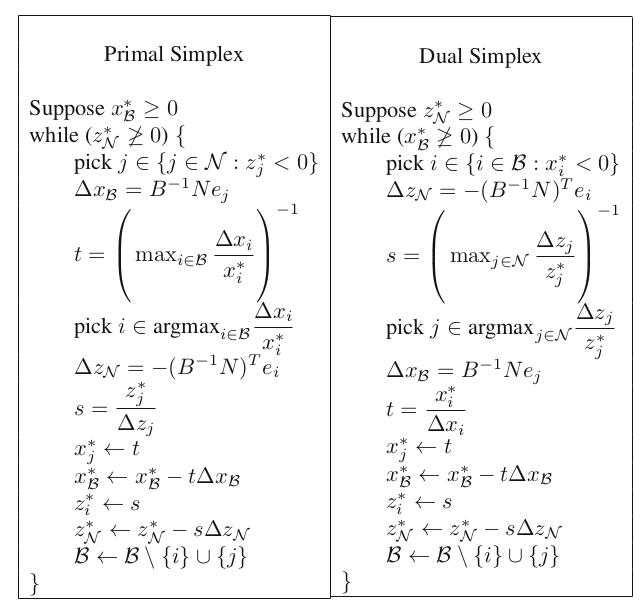
\includegraphics[width=.9\linewidth]{The Simplex Method in Matrix Notation/screenshot_2019-02-11_17-52-35.png}
\end{center}

\begin{itemize}
\item Instead of assuming that the primal dictionary is feasible one can use that the dual dictionary is feasible to perform the analogous steps
\end{itemize}

\section{Implementation Issues}
\label{sec:orgfe2bbfd}
\subsection{Introduction}
\label{sec:orgf5d605d}
\begin{itemize}
\item The most time-consuming steps in the simplex method are the computations
\end{itemize}
\begin{center}
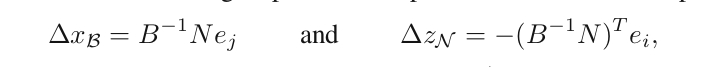
\includegraphics[width=.9\linewidth]{Implementation Issues/screenshot_2019-02-11_18-03-47.png}
\end{center}
\begin{itemize}
\item We dont compute the inverse of the basis matrix instead we calculate \(\Delta x_{\mathcal B}\) by solving the following system of equations
\end{itemize}
\begin{equation}
  B \Delta x_{\mathcal B} = a_j 
\end{equation}
where
\begin{equation}
  a_j = N e_j
\end{equation}
is the column of \(N\) associated with nonbasic variable \(x_j\) 
\begin{itemize}
\item The calculation of \(\Delta z_{\mathcal N}\) is also broken into two steps
\end{itemize}
\begin{align*}
	B^T v &= e_i  \\
	\Delta z_{\mathcal N} &= -N^T v
\end{align*}
\begin{itemize}
\item Solving the two systems of equation is where most of the complexity of the simplex iteration ies
\end{itemize}

\subsection{Solving Systems of Equations: \(LU\) Factorization}
\label{sec:orgddc9090}
\begin{itemize}
\item The systems of equation will be on the form
\end{itemize}
\begin{equation*}
  B x = b
\end{equation*}
where \(B\) is an invertible \(m \times m\) matrix and \(b\) is an arbitrary \(m\) vector

\begin{itemize}
\item If when doing Gaussian Elimination on a matrix \(B\) one saves the row before doing the operation then one obtains a matrix \(D\)
\begin{itemize}
\item One takes the matrix and splits it into three matrices
\begin{itemize}
\item \(D_1\) containing all elements on or below the diagonal
\item \(D_2\) One containing only the diagonal elements
\item \(D_3\) containing all elements on or above the diagonal
\end{itemize}
\item Then the following equation holds \(B=D_1 D_2^{-1} D_3\)
\item The following is denoted \(L\)
\end{itemize}
\end{itemize}
\begin{equation}
  L = D_1 D_2^{-1}
\end{equation}
\begin{itemize}
\item The following is denoted \(U\)
\end{itemize}
\begin{equation}
  U = D_3
\end{equation}
\begin{itemize}
\item The resulting representation \(B = LU\) is called an LU-factorization of \(B\)
\begin{itemize}
\item Finding an LU factorization is equivalent to Gaussian elimination since multiplying \(B\) on the left by \(L^{-1}\) has the effect of applying row operations to \(B\) to put it into upper-triangular form \(U\)
\end{itemize}

\item The value of an LU factorization can be used to solve systems of equations
\item If one wanted to solve \(B \Delta x_{\mathcal B} = a_j\)
\begin{itemize}
\item One first substitute \(LU\) for \(B\) so the system becomes \(LU \Delta x_{\beta} = a_j\)
\item If one lets \(y = U \Delta x_{\mathcal B}\) one can solve \(Ly=b\) for \(y\)
\begin{itemize}
\item Since \(L\) is lower triangular solving this equation is easy
\begin{itemize}
\item Successively solving for the elements of the vector \(y\) starting with the first and proceeding to the last is called \textbf{forward substitution}
\item This is an easy way to solve this
\end{itemize}
\end{itemize}
\item Once \(y\) is known one can solve \(U \Delta x_{\mathcal B} = y\) for \(\Delta x_ {\mathcal B}\)
\begin{itemize}
\item Since \(U\) is upper triangular solving this is easy as well
\item Successively solving for the elements of the vector \(\Delta x_{\mathcal B}\) starting with the last and back to the last is called \textbf{backward substitution}
\begin{itemize}
\item This is an easy way to solve this
\end{itemize}
\end{itemize}
\end{itemize}
\end{itemize}

\subsection{Exploiting Sparsity}
\label{sec:orgeded59c}
\begin{itemize}
\item A matrix that contains zeroes is called a \textbf{sparse matrix}
\item When a sparse matrix has lots of zeros two things happen
\begin{enumerate}
\item The changes of being required to make row and/or column permutations is high
\item Additional computation efficiency can be obtained by making further row and/or column permutation with the aim of keeping \(L\) and/or \(U\) as sparse as possible
\end{enumerate}

\item The problem with finding the "best" permutation is, in itself, harder than the linear programming problem
\item There are simple heuristics that help preserver sparsity in \(L\) and \(U\)
\begin{itemize}
\item One such heuristic called the \textbf{minimum-degree} ordering heuristic is as follows
\end{itemize}
\end{itemize}
\begin{center}
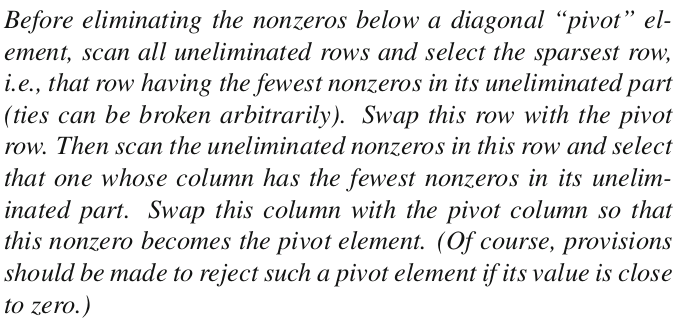
\includegraphics[width=.9\linewidth]{Implementation Issues/screenshot_2019-02-11_19-06-52.png}
\end{center}
\begin{itemize}
\item The number of non zeros in the uneliminated part of a row/column is called the \textbf{degree} of the row/column
\item The fact that the rows and columns to get this factorization has been permuted has only a small impact on how one uses the factorization to solve the systems of equations
\begin{itemize}
\item The first step is to permute the rows of the \(a_j\) so the fit the given permutation
\item Then one just does the same thing as before and in the end rewrite the solution to get the listing of elements in the original order
\item Since LU factorization is a \(m^3\) algorithm one should perform as few LU-factorizations as possible
\end{itemize}
\end{itemize}

\section{Integer Programming}
\label{sec:org38f33c3}
\subsection{Introduction}
\label{sec:org3060218}
\begin{itemize}
\item Many real-world problems could be modeled as linear programs except some or all the variables are constrained to be integers
\begin{itemize}
\item They are called \textbf{integer programming problems}
\item It is harder than linear programming
\end{itemize}
\end{itemize}

\subsection{Scheduling Problems}
\label{sec:org2ab22b2}
\begin{itemize}
\item There are many problems that can be classified as scheduling problems
\begin{itemize}
\item There are e.g. two related problems of this type the equipment scheduling and crew scheduling problem by large airlines
\end{itemize}

\item The equipment scheduling problem	
\begin{itemize}
\item Airlines determine how to route their planes as follows
\begin{enumerate}
\item A number of specific flight legs are defined based on market demand
\begin{itemize}
\item A leg is by definition one flight taking off from somewhere at some time and landing somewhere else
\item They are defined by market demand
\item One wants to put this legs together in such a way that the available aircraft can cover all of them
\begin{itemize}
\item For each airplane the airline must put together a route that it will fly
\end{itemize}
\item A route is a sequence of flight legs for which the destination of one leg is the origin or the next
\begin{itemize}
\item The final destination must be the origin of the first leg
\end{itemize}
\end{itemize}
\item Given potential routes one wants select a subset of them with the property that each leg is covered by exactly one route
\begin{itemize}
\item If there are enough potential routes there might be multiple feasible solutions
\item The goal is to find the optimal one
\item To formulate the problem as an integer program let
\end{itemize}
\end{enumerate}
\end{itemize}
\end{itemize}
\begin{center}
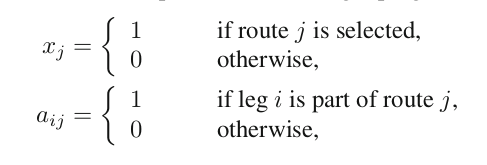
\includegraphics[width=.9\linewidth]{Integer Programming/screenshot_2019-02-17_09-23-44.png}
\end{center}
\begin{itemize}
\item and
\end{itemize}
\begin{center}

\includegraphics[width=.9\linewidth]{Integer Programming/screenshot_2019-02-17_09-24-19.png}
\end{center}
\begin{itemize}
\item Then the problem is
\begin{center}
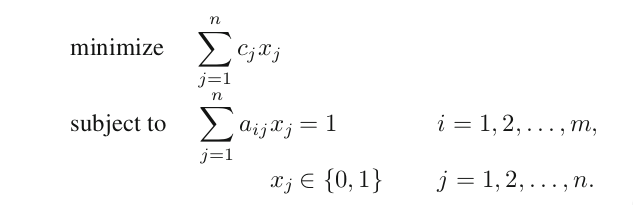
\includegraphics[width=.9\linewidth]{Integer Programming/screenshot_2019-02-17_09-24-46.png}
\end{center}
\item This model is often called a \textbf{set-partitioning problem}

\item The \textbf{crew scheduling problem}
\begin{itemize}
\item Flight crews do not necessarily follow the same aircraft around a route
\item The constraints differ from those for the aircraft
\item Flight crews might ride as passengers on some legs
\item The model is
\end{itemize}
\end{itemize}
\begin{center}
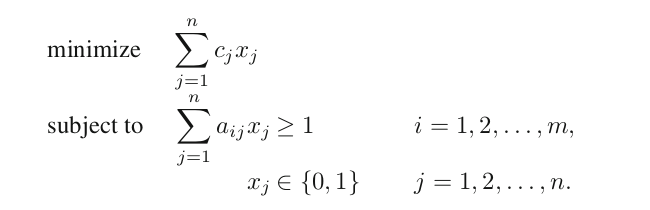
\includegraphics[width=.9\linewidth]{Integer Programming/screenshot_2019-02-17_09-28-48.png}
\end{center}
\begin{itemize}
\item Is often referred to as a \textbf{set-covering problem}
\end{itemize}

\subsection{The Traveling Salesman Problem}
\label{sec:orgd998bbf}
\begin{itemize}
\item Consider a salesman who needs to visit each of \(n\) cities
\begin{itemize}
\item They are enumerated as \(0,1,\dots, n-1\)
\item The goal is to start from his home city \(0\) and make a tour visiting each of the remaining cities once and only once and then returning to his home
\item The distance between each pair of cities \(c_{ij}\) is known
\begin{itemize}
\item It could also be travel time or cost of travel
\end{itemize}
\item He wants to make the tour that minimizes the total distances
\item The tour is determined by listing the cities in the order in which they will be visited
\begin{itemize}
\item If one let \(s_i\) denote the ith city visited the
\item The tour can be described as \(s_0 = 0, s_1, s_2, \dots, s_{n-1}\)
\end{itemize}
\item One can permute the cities in \((n-1)!\) possible ways and therefore the problem cannot be solved by enumeration
\item For each \((i,j)\) a decision variable \(x_{ij}\) is introduced that will be equal to one if the tour vists city \(j\) immediately after visiting city \(i\)
\begin{itemize}
\item Otherwise it will be equal to 0
\item The objective function can be written using these variables as minimize \(\sum_{i} \sum_{j} c_{ij} x_{ij}\)
\end{itemize}
\item If the salesman visits city \(i\) he must go to one and only one city next
\begin{itemize}
\item These constraints can be written as \(\sum_{j} x_{ij} = 1 \quad i=0,1,\dots,n-1\)
\item They are called \textbf{go-to constraints}
\end{itemize}
\item When the salesman visits a city he must have come from one and only one prior city i.e.
\begin{itemize}
\item \(\sum_{i} x_{ij} = 1 \quad j=0,1,\dots,n-1\)
\item They are called the \textbf{come-from constraints}
\end{itemize}
\item Let \(t_i\) for \(i=0,1,\dots, n\) be defined as the number of the stop along the tour for which city \(i\) is visited
\begin{itemize}
\item From this we see that \(t_{s_i} = i \quad i = 0,1,\dots,n-1\)
\item For a bonafide tour \(t_j = t_i +1\) if \(x_{ij} = 1\)
\item Each \(t_i\) is an integer between \(0\) and \(n-1\) inclusive
\item \(t_j\) satisfies the following constraints
\end{itemize}
\end{itemize}
\end{itemize}
\begin{center}
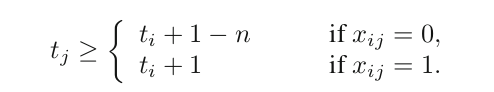
\includegraphics[width=.9\linewidth]{Integer Programming/screenshot_2019-02-17_10-03-58.png}
\end{center}
\begin{itemize}
\item The constraints can be written succinctly as
\end{itemize}
\begin{center}
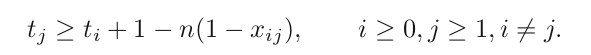
\includegraphics[width=.9\linewidth]{Integer Programming/screenshot_2019-02-17_10-05-04.png}
\end{center}
\begin{itemize}
\item The constraints forces a solution to be a bonafide tour
\end{itemize}
\begin{itemize}
\item The traveling salesman problem can be formulated as the following integer programming problem
\end{itemize}
\begin{center}
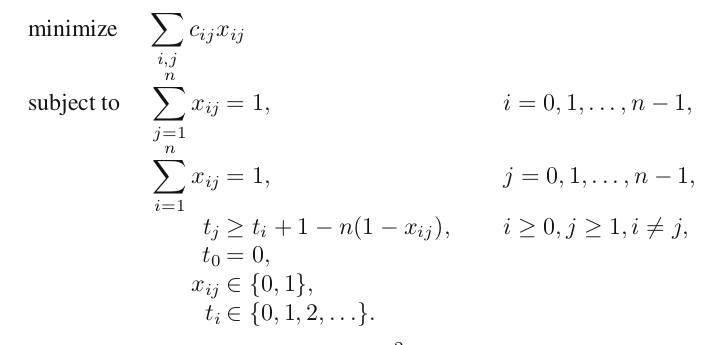
\includegraphics[width=.9\linewidth]{Integer Programming/screenshot_2019-02-17_10-06-38.png}
\end{center}

\subsection{Fixed Costs}
\label{sec:orgbfc649c}
\begin{itemize}
\item It is sometimes more realistic to assume that there is a fixed cost for engaging in the activity plus a linear variable cost
\begin{itemize}
\item Such a term might have the form
\end{itemize}
\end{itemize}
\begin{equation*}
  c(x) =
    \begin{cases}
      \mbox{$0$} & \mbox{if $x=0$} \\
      \mbox{$K + cx$} & \mbox{if $x>0$}
    \end{cases}
\end{equation*}
\begin{itemize}
\item If there is an upper bound on the size of \(x\) such a function can be equivalently modeled using strictly linear functions at the expense of introducing one integer-valued variable
\begin{itemize}
\item Suppose \(u\) is an upper bound on the \(x\) variable
\item Let \(y\) denote a \(\{0,1\}\) valued variable which is one when and only when \(x > 0\)
\item Then \(c(x) = Ky + cx\)
\item The condition that \(y\) is one exactly when \(x>0\) can be guaranteed by introducing the following constraints
\end{itemize}
\end{itemize}
\begin{align*}
  x \leq uy \\
  x \geq 0 \\
  y \in \{0,1\} 
\end{align*}

\subsection{Nonlinear Objective Functions}
\label{sec:org125aff5}
\begin{center}
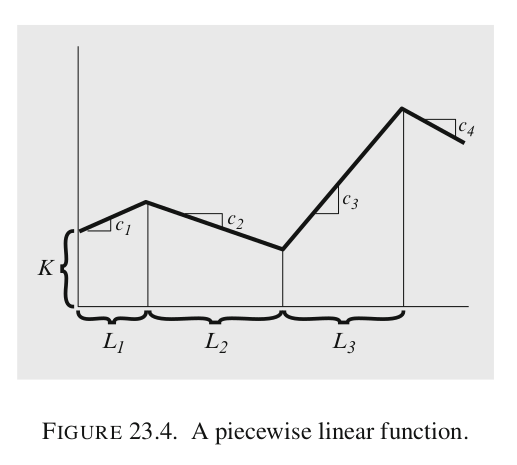
\includegraphics[width=.9\linewidth]{Integer Programming/screenshot_2019-02-17_10-28-30.png}
\end{center}

\begin{itemize}
\item Sometimes the terms in the objective function are not linear at all
\begin{itemize}
\item Formulating an integer programming approximation to a general nonlinear term in the objective function is done in the following way
\begin{enumerate}
\item Approximate the nonlinear function by a continuous piecewise linear function
\item Introduce integer variables that allow us to represents the piecewise linear function using linear relations
\begin{itemize}
\item We decompose the variable \(x\) into a sum: \(x=x_1+x_2+ \dots + x_k\)
\item \(x_i\) denotes how much of the interval \([0,x]\) is contained in the ith linear segment of the piecewise linear function
\item Constraints are needed to guarantee
\begin{itemize}
\item That the initial \(x_i\)'s are equal to the length of their respective segments
\item That after the straddling segment the subsequent \(x_i\)'s are all zero
\item The following constraints do the trick:
\end{itemize}
\end{itemize}
\end{enumerate}
\end{itemize}
\end{itemize}
\begin{center}
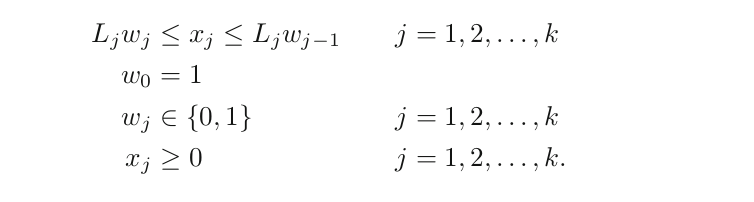
\includegraphics[width=.9\linewidth]{Integer Programming/screenshot_2019-02-17_10-26-18.png}
\end{center}

\begin{itemize}
\item It follows from the constrains that \(w_j \leq w_{j-1}\) for \(j=1,2,\dots,k\)
\begin{itemize}
\item This inequality implies that once one of the \(w_j\) is zero all the subsequent once must be zero
\item With this decomposition we can write the piecewise linear function as
\end{itemize}
\end{itemize}
\begin{equation}
  K + c_1x_1 + c_2x_2 + \dots + c_k x_k
\end{equation} 

\subsection{Branch-and-Bound}
\label{sec:org3cdc8f7}
\begin{itemize}
\item The standard \textbf{integer programming problem} is defined as follows:
\end{itemize}
\begin{center}
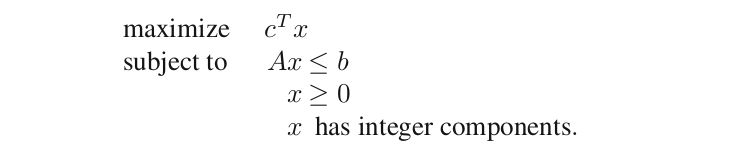
\includegraphics[width=.9\linewidth]{Integer Programming/screenshot_2019-02-17_10-35-32.png}
\end{center}

\begin{itemize}
\item The algorithm called \textbf{branch-and-bound} solves the standard integer problem
\begin{itemize}
\item It starts out with the following wishful approach
\begin{enumerate}
\item First ignore the constraint that the components of \(x\) be integers
\item Solve the resulting linear programming problem
\item Hope that the solution vector has all integer components
\end{enumerate}
\item Hopes are almost always unfulfilled so a backup strategy is needed
\item The simplest strategy of rounding down the numbers do not always work
\begin{itemize}
\item The numbers might not be feasible
\end{itemize}
\item The linear programming problem obtained by dropping the integrality constraint is called the \textbf{LP-relaxation}
\begin{itemize}
\item Since it has fewer constraints its optimal solution provides an upper bound \(\zeta^0\) on the optimal solution \(\zeta^*\)
\end{itemize}
\end{itemize}
\end{itemize}

\begin{center}
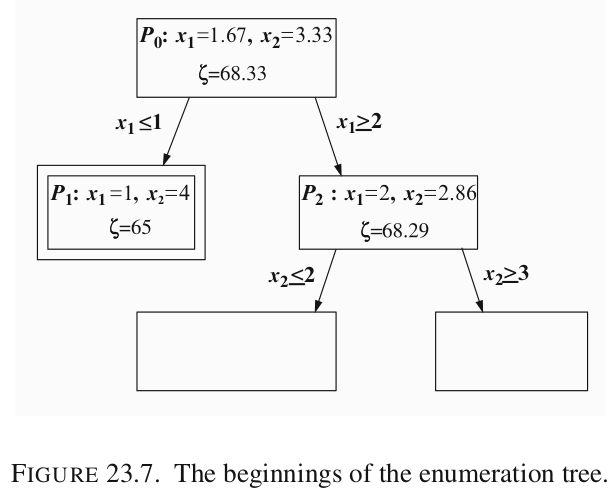
\includegraphics[width=.9\linewidth]{Integer Programming/screenshot_2019-02-17_10-58-30.png}
\end{center}
\begin{itemize}
\item The algorithm works as follows
\begin{itemize}
\item Solve the problem using the simplex algorithm
\begin{enumerate}
\item If the solution is an integer solution check if it is greater than the current best solution
\item Else if the value is greater than the current best solution split the problem into to for the first non-integer variable
\begin{itemize}
\item e.g. if \(x_i = 3.1\) we split into to problems one with \(x_i \leq 3\) and one with \(x_i \geq 4\)
\item Solve the left problem first by going to step 1 and then the right problem
\item This is done using a enumeration tree
\end{itemize}
\end{enumerate}
\end{itemize}

\item Reasons for using depth first search
\begin{enumerate}
\item Most integer solutions lie deep in the three there are two advantages to finding the integer feasible solutions early 
\begin{enumerate}
\item It is better to have a feasible solution than nothing in case one wishes to abort the solution process early
\item Identifying a feasible integer solution can result in subsequent nodes of the enumaration tree begin made into leaves
\begin{itemize}
\item This isbecause the optimal objective function associated with the nodes is lower than the best so-far integer solution
\end{itemize}
\end{enumerate}
\item The facts that it is very easy to code the algorithm as a recursive defined function
\item As one moves deeper in the enumaration tree each subsequent linear problem is obtained from the preceding one by simply adding an upper/lower bound on one specific variable
\end{enumerate}
\end{itemize}

\section{Network Flows}
\label{sec:org98f9e6d}
\subsection{Totally unimodular linear programs}
\label{sec:orgab2ed79}
\subsubsection{The assignment problem}
\label{sec:org4f4bf65}
\begin{itemize}
\item There is given a \(n \times n\) matrix of matrix of costs \(C=(c_{ij})\)
\item The goal is to find a permutation \(\pi\) on \(\{1,2, \dots, n\}\) minimizing \(\sum_{i=1}^n c_{i,\pi(i)}\)
\item The following \(n^2\) decision variables is chosen
\end{itemize}
\begin{center}

\includegraphics[width=.9\linewidth]{Network Flows/screenshot_2019-02-24_14-17-45.png}
\end{center}

\begin{itemize}
\item The problem can be formulated as an integer LP problem as follows:
\end{itemize}
\begin{center}
\includegraphics[width=.9\linewidth]{Network Flows/screenshot_2019-02-24_14-18-01.png}
\end{center}
\begin{itemize}
\item Solving this problem by using the simplex algorithm without the integral constraint always gives us an integral solution
\end{itemize}

\subsubsection{Cramer's rule and matrix determinants}
\label{sec:orgf8704ac}
\begin{itemize}
\item Let \(A= (a_{ij})\) be a \(m \times m\) matrix, \(b \in \mathbb R^m\) and consider the linear system
\end{itemize}
\begin{equation}
  Ax = b
\end{equation}
\begin{itemize}
\item When the system has a unique solution it can be found using Cramer's rule

\item \textbf{Theorem 1.} (Cramer's rule) The system has a unique solution if and only if \(det(A) \ne 0\) and in that case it is given by
\end{itemize}
\begin{equation}
  x_i = \frac{\det{(A_i)}}{\det{A}}
\end{equation}
where \(A_i\) is obtained from \(A\) by replacing column \(i\) by the vector \(b\) 

\begin{itemize}
\item \textbf{Observation 1.} Given that all entries of \(A\) and \(b\) are integers. Then \(\det(A_i)\) is an integer for all \(i\) Now, a sufficient condition for \(x_i\) to be integer for all i is that \(\det(A) \in {-1,1}\)

\item \textbf{Proposition 1.} (Laplace's formula) Let \(A = (a_{ij})\) be a \(m \times m\) matrix. Then
\end{itemize}
\begin{center}
\includegraphics[width=.9\linewidth]{Network Flows/screenshot_2019-02-24_14-37-12.png}
\end{center}
where \(A_{ij}\) is the \((m-1) \times (m-1)\) matrix obtained from \(A\) by removing row \(i\) as well as column \(j\)

\begin{itemize}
\item \textbf{Proposition 2.} Let \(A\) be a \(m \times m\) matrix. Then
\begin{enumerate}
\item If \(B\) is obtained from \(A\) by exchanging two rows or two columns then \(\det(B) = -\det(A)\)
\item If \(B\) is obtained from \(A\) my multiplying a row or a column by \(c\), then \(\det(B) = c \det(A)\)
\item If \(B\) is obtained from \(A\) by adding a multiple of a row to another row or by adding a multiple of a column to another column, then \(\det(B) = \det(A)\)
\end{enumerate}
\end{itemize}

\subsubsection{Totally unimodular matrices}
\label{sec:orgfba151b}
\begin{itemize}
\item \textbf{Definition 1.} A matrix \(A\) is \textbf{totally unimodular} if every square submatrix of \(A\) has determininant either 0, 1 or -1
\item \textbf{Theorem 2} (Hoffman and Kruskal's Theorem). Let \(A\) be an integer \(m \times n\) matrix
\begin{itemize}
\item \(A\) is totally unimodular if and only if for every integer vector \(b \in \mathbb Z^m\) all the basic solutions of \(F = \{ Ax \leq b, x \geq 0\}\) are integer
\end{itemize}
\item \textbf{Theorem 3.} Let \(A= (a_{ij})\) be a totally unimodular \(m \times n\) matrix and let \(b \in \mathbb Z^m\). Then every basic solution of \(F = \{A \leq b, x \geq 0\}\) is integer
\item A linear program in standard form is called for totally unimodular if the coefficient matrix \(A\) is totally unimodular and the vector of constants \(b\) is integer valued
\begin{itemize}
\item A desirable property since for many real life problems one is interested in integer solutions
\end{itemize}

\item \textbf{Lemma 1.} If \(A\) is a matrix with entries from \(\{-1,0,1\}\) with the property that each column contains at most two non-zero entries, at most one being \(1\) and at most one being \(-1\) then \(A\) is totally unimodular
\item \textbf{Lemma 2.} Let \(A\) be totally unimodular.
\begin{itemize}
\item Then \(A^T\) is totally unimodular.
\item Let \(B\) be obtained from \(A\) by removing rows or columns, by exchanging rows, by exchanging columns, or by multiplying rows or columns by \(-1\). Then \(B\) is also totally unimodular
\end{itemize}
\item \textbf{Lemma 3.} Let \(A\) be totally unimodular. Then \([A \quad I]\) and \([A \quad A]\) are totally unimodular
\end{itemize}

\subsection{Networks}
\label{sec:orgb2e0372}
\subsubsection{General}
\label{sec:org4690172}
\begin{itemize}
\item A \textbf{flow network} or simply a \textbf{network} is a directed graph \(D = (\mathcal N, \mathcal A)\)
\begin{itemize}
\item A \textbf{flow} in a network is an assignment of a real number to each arc, the \textbf{flow} on the arc
\begin{itemize}
\item One may thus think of a flow as a function \(x: \mathcal A \rightarrow \mathbb R\)
\item One typically view the flow as an assignment to variables \(x_{ij}\) for each \(ij \in A\)
\end{itemize}
\item Various \textbf{constraints} can be imposed onto flow networks
\begin{itemize}
\item There is always a nonnegative constraint, stating that \(x_{ij} \geq 0\) for all \(ij \in A\)
\item Additional constraints that one can consider are \textbf{balance constraints} and arc \textbf{capacity constraints}
\item A flow that satisfies all given constraints is called a \textbf{feasible} flow
\end{itemize}
\item It is often built to model a real-life network
\begin{itemize}
\item Much terminology is borrow from real life networks
\end{itemize}
\item For a node \(i \in \mathcal N\) the \textbf{outgoing flow} from \textbf{i} is given by the summation of flow on all outgoing arcs from \(i\), \(\sum_{ij \in A} x_{ij}\)
\item The \textbf{ingoing flow} from \(i\) is given by the summation of flow on all ingoing arcs to \(i\), \(\sum_{ji \in A} x_{ji}\)
\item The \textbf{balance} of node \(i\) with respect to the flow \(x\) is given by the difference of the outgoing flow and the ingoing flow
\end{itemize}
\end{itemize}
\begin{equation}
  b_i(x) = \sum_{ij \in a} x_{ij} - \sum_{ji \in a} x_{ji}
\end{equation}
\begin{itemize}
\item Flow is supplied at a node \(i\) if \(b_i(x) > 0\) we call \(i\) a \textbf{source} node
\item Flow is consumed at a node \(i\) if \(b_i(x) < 0\) we call \(i\) a \textbf{sink} node
\item If a flow has no sources or sinks we call the flow a \textbf{circulation}
\end{itemize}

\subsubsection{Node balance constraints}
\label{sec:org6a71b8b}
\begin{itemize}
\item A balance constraint is specified by balances \(b_i\) for each \(i \in \mathcal N\) and states that
\end{itemize}
\begin{equation}
 	b_i(x) = b_i 
\end{equation} 
for all \(i \in \mathcal N\)
\begin{itemize}
\item It is necessary to have \(\sum_{i \in \mathcal N} b_i = 0\) in  order to have feasible flows which always is an asumption when we have a balance constraint
\item This means we always have
\end{itemize}
\begin{center}
\includegraphics[width=.9\linewidth]{Network Flows/screenshot_2019-02-27_13-17-15.png}
\end{center}

\subsubsection{Arc constraints}
\label{sec:orgce64555}
\begin{itemize}
\item Arc constraint are specified by \textbf{upper bounds} \(u_{ij}\) (also called capacities) and lower bounds \(l_{ij}\) for each \(ij \in \mathcal A\) and states that
\end{itemize}
\begin{equation}
  l_{ij} \leq x_{ij} \leq u_{ij}
\end{equation}
for all \(ij \in \mathcal A\)
\begin{itemize}
\item It is also necessary to have \(0 \leq l_{ij} \leq u_{ij}\) for all \(ij \in \mathcal A\) to have feasible flows
\item When only upper bounds is specified we implicitly assume \(l_{ij} = 0\) for all \(ij \in \mathcal A\)
\end{itemize}

\subsection{The minimum cost flow problem}
\label{sec:org44f73f5}
\subsubsection{General}
\label{sec:org6eb6a42}
\begin{itemize}
\item The minimum cost flow problem is to minimize the \textbf{cost} of a flow in a network subject to certain given constraints
\begin{itemize}
\item The most basic cost model is a linear cost model that assigns a real-valued cost \(c_{ij}\) to each arc \(ij \in A\)
\begin{itemize}
\item The cost of an arc represents the cost per unit flow along that arc
\item It is also allowed to be a negative number
\end{itemize}
\item The cost of a given flow \(x\) is given by
\end{itemize}
\end{itemize}
\begin{equation}
 	c(x) = \sum_{ij \in \mathcal A} c_{ij}x_{ij} 
\end{equation}
\begin{itemize}
\item In the minimum cost flow problem we are always given balance constraints
\item Capacity constraints are optional
\end{itemize}

\subsubsection{Integrality theorem}
\label{sec:orgb5c7473}
\begin{itemize}
\item \textbf{Theorem 4.} Let \(D = (\mathcal N, \mathcal A)\) be a network 
\begin{itemize}
\item with costs given by \(c_{ij} \in \mathbb R\)
\item with balance constraints given by \(b_i \in \mathbb Z \text{ for } i \in \mathcal N\)
\item with lower and upper bounds given by \(l_{ij}, u_{ij} \in \mathbb Z\) where \(0 \leq l_{ij} \leq u_{ij}, \text{ for } ij \in \mathcal A\)
\item Then there is a minimum cost feasible flow \(x\) with an integer valued flow on every arc
\end{itemize}
\end{itemize}

\subsection{The maximum \((s,t)\) flow problem}
\label{sec:org02db5f4}
\subsubsection{General}
\label{sec:org8805d46}
\begin{itemize}
\item The \((s, t)\) flow problem may be viewed as a important special case of the minimum cost flow problem
\begin{itemize}
\item One is given a flow network \(D=(\mathcal N, \mathcal A)\) with specified upper bound, together with two nodes \(s,t \in \mathcal N\) being singled out
\item The node \(s\) is thought of as a source node
\item The node \(t\) is thought of as a sink node
\item The \textbf{flow conservation} constraint states that \(b_i(x) = 0\) for all \(i \in \mathcal N \backslash \{s,t\}\)
\item A flow is feasible if it satisfies
\begin{itemize}
\item The non-negativity constraint
\item The flow conservation constraint
\item The arc constraint given by the upper bounds
\end{itemize}
\item For a feasible we define the \textbf{value} as \(|x| = b_s(x)\)
\item The maximum \((s,t)\) flow problem is to find a feasible flow \(x\) maximizing the value \(|x|\)
\end{itemize}

\item To model the maximum \((s,t)\) flow problem as a minimum cost flow problem the following is done
\begin{itemize}
\item Given a network \(D=(\mathcal N, \mathcal A)\) with a specified source \(s\) and sink \(t\) we add to \(\mathcal A\) an arc from \(t\) to \(s\) obtaining the new network \(D'\)
\item We state the minimum cost flow problem on \(D'\) by given the new arc from \(t\) to \(s\) cost \(-1\) and upper bound \(\infty\)
\item All other arcs are given cost \(0\)
\item All nodes are given balance \(0\)
\item Feasible flows \(x\) in \(D\) corresponds to feasible flows \(x'\) in \(D'\) where the cost of \(x'\) is the negative of the value of \(x\)
\end{itemize}
\end{itemize}

\subsubsection{The max-flow min-cut theorem}
\label{sec:orgbeac30f}
\begin{itemize}
\item A reason for the importance of the maximum \((s,t)\) flow problem is the celebrated max-flow min-cut theorem
\item An \((s,t)\) cut of \(D\) is a partition \((S,T)\) of the nodes of \(D,\mathcal N = S \cup T\) such that \(s \in S\) and \(t \in T\)
\begin{itemize}
\item The \textbf{capacity} \(u(S,T)\) of a \((s,t)\) cut \((S,T)\) is given by
\end{itemize}
\end{itemize}
\begin{center}
\includegraphics[width=.9\linewidth]{Network Flows/screenshot_2019-02-27_14-23-14.png}
\end{center}
\begin{itemize}
\item The minimum capacity \((s,t)\) cut problem is the associated minimization problem of finding a \((s,t)\) cut of minimum capacity
\end{itemize}
\begin{itemize}
\item \textbf{Theorem 5} (Max-flow min-cut Theorem). Let \(x\) be a flow of maximum value and let \((S,T)\) be a \((s,t)\) cut of minimum capacity. Then
\end{itemize}
\begin{equation}
  |x| = u(S,T)
\end{equation}

\subsection{Solving the minimum cost flow problem}
\label{sec:org4bef2b5}
\subsubsection{Introduction}
\label{sec:org51c9a53}
\begin{itemize}
\item The two basic assumptions placed on networks are the following
\begin{enumerate}
\item The network is connected when viewed as an undirected graph
\item The network does not contain any 2-cycles
\begin{itemize}
\item i.e. if \(ij\) is an arc then the arc \(ji\) is not present in the network
\end{itemize}
\end{enumerate}

\item If the graph is not connected one can just solve the minimum cost flow problem for each graph and then combine them
\item The two cycles assumption is only made for clarity of presentation
\begin{itemize}
\item The algorithm considered work even in the presence of 2 cycles
\item One can eliminate 2 cycles by subdividing one of the arcs introducing an auxiliary node
\end{itemize}
\end{itemize}
\begin{center}
\includegraphics[width=.9\linewidth]{Network Flows/screenshot_2019-03-03_14-26-34.png}
\end{center}

\subsubsection{Transformation to uncapacitated networks}
\label{sec:org5e6d3f6}
\begin{itemize}
\item Transforming a network with arc-constraints to an uncapacitated network can be done by introducing an auxiliary node for each arc adjusting balances
\begin{itemize}
\item An arc \(ij\) with lower bound \(l_{ij}\), upper bound \(u_{ij}\) and cost \(c_{ij}\) with arcs from is replaced with arcs from node \(i\) and \(j\) to an auxilary node \(j_{ij}\) with the balance \(l_{ij} - u_{ij}\)
\item The cost of the arc \((i,l_{ij})\) becomes \(c_{ij}\) and the cost of the arc \((k_{ij}, i)\) becomes \(0\)
\item A flow \(x\) in the original network corresponds to the flow \(x'\) in the transformed network letting \(x'_{i,k_{ij}} = x_{ij} - l_{ij}\) and \(x'_{j,k_{ij}} = u_{ij} - x_{ij}\)
\item A flow \(x'\) in transformed network corresponds to to the flow \(x\) in the original network letting \(x_{ij} = x'_{i,k_{ij}} + l_{ij}\)
\item The cost of the two flows are related by a constant difference \(c(x') = c(x) - \sum_{ij \in \mathcal A} l_{ij} c_{ij}\)
\end{itemize}
\end{itemize}

\begin{center}
\includegraphics[width=.9\linewidth]{Network Flows/screenshot_2019-03-03_14-40-47.png}
\end{center}

\begin{itemize}
\item This transformation can be used on the general network, so one can use the algorithm from the book
\end{itemize}

\subsubsection{Klein's cycle cancelling algorithm}
\label{sec:org46cfa48}
\begin{enumerate}
\item General
\label{sec:org262341b}
\begin{itemize}
\item The general case of a network \(D= (\mathcal N, \mathcal A)\) is considered with balances \(b_i\) lower bounds \(l_{ij}\), upper bounds \(u_{ij}\) and costs \(c_{ij}\)

\item The cycle cancellation algorithm abandons the restriction to tree solution and allows any cycle in the network to be a candidate for improving the cost the current flow
\begin{itemize}
\item If no cycle can be found that improves the network the algorithms terminates and returns the current solution
\item A \textbf{cycle} \(C\) in \(D\) will be a simple cycle in \(D\) when viewed as an undirected graph together with a direction
\begin{itemize}
\item \(C\) is just a sequence of nodes \(i_1,i_2,\dots,i_\ell \in \mathcal N\) with \(i_\ell = i_1\) butt all other \(i_k\) being different and such that either
\begin{enumerate}
\item \((i_k,i_{k+1}) \in \mathcal A\) for all \(k=1, \dots, \ell-1\) which is called a \textbf{forward edge} of \(C\)
\item \((i_{k+1}, i_k) \in \mathcal A\) for all \(k=1, \dots, \ell-1\) which is called a \textbf{backward edge} of \(C\)
\end{enumerate}
\end{itemize}
\item Let \(C\) be a cycle in \(D\)
\begin{itemize}
\item Let \(F\) be the set of forward edges of \(C\) and
\item Let \(B\) be the set of backward edges of \(C\)
\item The cost \(c(C)\) of the cycle \(C\) is defined as
\end{itemize}
\end{itemize}
\end{itemize}
\begin{equation}
  c(C) = \sum_{ij \in F} c_{ij} - \sum_{ij\in B} c_{ij}
\end{equation}
\begin{itemize}
\item Given a real number \(\delta\), define the cycle flow \(\gamma_C^\delta\) as
\end{itemize}
\begin{equation*}
  \gamma_C^\delta =
    \begin{cases}
      \mbox{$\delta$} & \mbox{if $ij \in F$} \\
      \mbox{$-\delta$} & \mbox{if $ij \in B$} \\
      \mbox{$0$} & \mbox{otherwise} 
    \end{cases}
\end{equation*}

\begin{itemize}
\item \textbf{Observation 2.} Let \(C\) be a cycle in \(D\)
\begin{enumerate}
\item The flow \(\gamma_C^\delta\) is a circulation. That is \(b_i(\gamma_C^\delta) = 0\) for all \(i \in \mathcal N\)
\item The cost of \(\gamma_C^\delta\) is given by \(c(\gamma_C^\delta) = \delta \cdot c(C)\)
\end{enumerate}

\item \textbf{Definition 2.} Let \(x\) be a feasible flow in \(D\) and let \(C\) be a cycle in \(D\). Then \(C\) is an \textbf{augmenting cycle} relative to \(x\) if \(c(C)<0\) and there exists \(\delta > 0\) such that \(x+\gamma_C^\delta\) is a feasible flow in \(D\)

\item When \(C\) is a cycle such that \(c(C) < 0\). Then \(C\) is an augmenting cycle relative to \(x\) if and only if \(x_{ij} < u_{ij}\) for all \(ij \in F\) and \(l_{ij} < x_{ij}\) for all \(ij \in B\).
\begin{itemize}
\item When \(C\) is an augmenting cycle, the maximum \(\delta >0\) for which \(x + \gamma_C^\delta\) remains a feasible flow, which we will denote by \(\delta(C)\) given by
\end{itemize}
\end{itemize}
\begin{center}
\includegraphics[width=.9\linewidth]{Network Flows/screenshot_2019-03-03_19-50-07.png}
\end{center}

\begin{itemize}
\item Outline of Klein's cycle cancelling algorithm
\end{itemize}
\begin{center}
\includegraphics[width=.9\linewidth]{Network Flows/screenshot_2019-03-03_19-50-37.png}
\end{center}
\item Finding the first feasible flow
\label{sec:orgaba54ec}
\begin{center}
\includegraphics[width=.9\linewidth]{Network Flows/screenshot_2019-03-04_20-57-12.png}
\end{center}

\begin{itemize}
\item The problem is formulated as a maximum flow problem
\begin{itemize}
\item It can be solved by Ford-Fulkerson or Edmonds-Karp algorithm
\item Given a flow network \(D=(\mathcal N, \mathcal A)\) a new flow network \(D' = (\mathcal N', \mathcal A')\) is build
\begin{itemize}
\item \(\mathcal N' = \{s,t\} \cup \mathcal N \cup \{k_{ij}^\ell \mid ij \in \mathcal A, \ell = 1,2\}\)
\item The arcs \(\mathcal A'\) of the network \(D'\) corresponds to the nodes and arcs of \(D\)
\item The arcs in \(D'\) corresponding to the nodes of \(D\) are as follows
\begin{itemize}
\item From \(s\) we have an arc to each \(i \in \mathcal N\) for which \(b_i > 0\)
\item To \(t\) we have an arc from each \(i \in \mathcal N\) for which \(b_i < 0\)
\end{itemize}
\item The arcs in \(D'\) corresponding to arcs \(ij \in \mathcal A\) are as follows
\begin{itemize}
\item We have arcs forming a path from \(i\) to \(j\) through nodes \(k_{ij}^1\) and \(k_{ij}^2\)
\item We have an arc from \(s\) to \(k_{ij}^2\) and an arc from \(k_{ij}^1\) to \(t\)
\end{itemize}
\item An arc from \(s\) to \(i\) is given upper bound \(b_i\)
\item An arc from \(i\) to \(t\) is given upper bound \(-b_i\)
\item The arcs from \(i\) to \(k_{ij}^1\) and from \(k_{ij}^2\) is given upper bounds \(u_ij\)
\item The arcs from \(s\) to \(k_{ij}^2\) and from \(k_{ij}^1\) to \(t\) are given upper bound \(l_{ij}\)
\item \(D\) has a feasible flow if and only if \(D'\) has a \((s,t)\) flow \(x'\) that saturates all arcs from the source \(s\)
\end{itemize}
\end{itemize}
\end{itemize}

\item Finding an augmenting cycle
\label{sec:org97d6302}
\begin{itemize}
\item The problem of finding an augmenting cycle is reduced to finding a negative weight directed cycle in a weighted directed graph
\item Let \(D=(\mathcal N, \mathcal A)\) be a network with balances \(b_i\), lower bounds \(l_{ij}\), upper bounds \(u_{ij}\) and costs \(c_{ij}\)
\item Let \(x\) be a feasible flow in \(D\)
\item The residual network relative to \(x\) is the network \(D_x=(\mathcal N, \mathcal A_x)\)
\begin{itemize}
\item It has the same set of nodes as \(D\)
\item The set of arcs indicates how the flow \(x\) may be changed maintaining feasibility
\item The arcs \(\mathcal A_x\) of \(D_x\) are given by
\end{itemize}
\end{itemize}
\begin{center}
\includegraphics[width=.9\linewidth]{Network Flows/screenshot_2019-03-07_09-07-13.png}
\end{center}
\begin{itemize}
\item Each arc \(ij \in \mathcal A\) of \(D\) can give rise to \(0,1\) or \(2\) arcs of \(D_x\) between the nodes \(i\) and \(j\)
\item When \(x_{ij} < u_{ij}\) the arc \(ij \in A_x\) is given upper bound \((u_x)_{ij} = u_{ij} - x_{ij}\)
\begin{itemize}
\item This specifies how much the flow on arc \(ij\) can be increased
\item It is given cost \((c_x)_{ij} = c_{ij}\)
\end{itemize}
\item When \(l_{ij} < x_{ij}\) the arc \(ji \in \mathcal A_x\) is given upper bound \((u_x)_{ji} = x_{ij} - l_{ij}\)
\begin{itemize}
\item This specifies how much the flow on arc \(ij\) can be decreased
\item It is given cost \((c_x)_{ji} = -c_{ij}\)
\end{itemize}
\item These upper bounds is called \textbf{residual capacities}
\item The balances of all nodes are set to \(0\)
\item All the arcs of \(D_x\) is given lower bound \(0\)

\item Let \(x\) and \(y\) be feasible flow in \(D\)
\begin{itemize}
\item The flow \(z = y-x\) in \(D\) is a circulation
\item The corresponding flow \(\tilde z\) in \(D_x\) is defined by giving positive flow according to the following rules
\begin{itemize}
\item If \(z_{ij} > 0\) we let \(\tilde z_{ij} = z_{ij}\) it also implies \(x_{ij} < y_{ij} \leq u_{ij}\) which means that the arc \(ij\) is present in \(D_x\)
\item If \(z_{ij} < 0\) we let \(\tilde z_{ji} = -z_{ij}\) it also implies \(x_{ij} > y_{ij} \geq l_{ij}\) which means that the arc \(ji\) is present in \(D_x\)
\end{itemize}
\item Arcs of \(D_x\) not assigned flow by these rules are given flow \(0\)
\item \textbf{Lemma 4.} \(\tilde z\) is a feasible flow in \(D_x\) and \(c_x(\tilde z) = c(z) = c(y) - c(x)\)
\end{itemize}

\item Let \(x\) be a feasible flow in \(D\), and let \(\tilde z\) be a feasible flow in \(D_x\)
\begin{itemize}
\item Define the flow \(z\) in \(D\) by the following rules specifying the flow \(z_{ij}\) on arc \(ij \in \mathcal A\)
\begin{itemize}
\item If \(ij \in \mathcal A_x\) and \(ji \in \mathcal A_x\) let \(z_{ij} = \tilde z_{ij} - \tilde z_{ji}\)
\item If \(ij \in \mathcal A_x\) and \(ji \notin \mathcal A_x\) let \(z_{ij} = \tilde z_{ij}\)
\item If \(ij \notin \mathcal A_x\) and \(ji \in \mathcal A_x\) let \(z_{ij} =  - \tilde z_{ji}\)
\end{itemize}
\item Let \(y = x+z\)
\item \textbf{Lemma 5.} \(y\) is a feasible flow in \(D\) and \(c(y) = c(x) + c(z) = c(x) + c_x (\tilde z)\)
\end{itemize}

\item The problem of finding an augmenting cycle in \(D\) relative to \(x\) is precisely the problem of finding a negative weight directed cycle in \(D_x\) when using the costs as weights
\end{itemize}

\item Partial correctness
\label{sec:org012f021}
\begin{center}
\includegraphics[width=.9\linewidth]{Network Flows/screenshot_2019-03-07_09-30-56.png}
\end{center}
\begin{center}
\includegraphics[width=.9\linewidth]{Network Flows/screenshot_2019-03-07_09-33-13.png}
\end{center}
\end{enumerate}

\section{Network Flow Problems}
\label{sec:org417d23f}
\subsection{Spanning Trees and Bases}
\label{sec:org128f918}
\begin{itemize}
\item An ordered list of nodes \((n_1,n_2,\dots,n_k)\) is called a \textbf{path} in the network if each adjacent pair of nodes in the list is connected by an arc in the network
\begin{itemize}
\item It is not assumed that the arcs point in any particular direction
\end{itemize}
\item A network is called connected if there is a path connecting every pair of nodes
\item For any arc \((i,j)\) \(i\) is its \textbf{tail} and \(j\) is its \textbf{head}
\item A \textbf{cycle} is a path in which the last node coincides with the first node
\item A network is called \textbf{acyclic} if it does not contain cycles
\item A network is a \textbf{tree} if it is connected and acyclic
\item A network \((\tilde{\mathcal N}, \tilde{\mathcal A})\) if called a \textbf{subnetwork} of \((\mathcal N, \mathcal A)\) if \(\tilde{\mathcal N} \subset \mathcal N\) and \(\tilde{\mathcal A} \subset \mathcal A\)
\begin{itemize}
\item It is a \textbf{spanning tree} if it is a tree and \(\tilde{\mathcal N} = \mathcal N\)
\item It is suffices to refer to a spanning tree by simply giving the arc set
\end{itemize}
\item Given a network flow problem any selection of primal flow values that satisfies the balance equations at every node is called a \textbf{balanced flow}
\begin{itemize}
\item If all flows are nonnegative the a it is called a \textbf{feasible flow}
\end{itemize}
\item Given a spanning tree, a balance flow that assigns zero flow to every arc not on the spanning tree is called a \textbf{tree solution}

\item It is assumed that the network is connected
\begin{itemize}
\item \textbf{Theorem} A square submatrix of \(\tilde{A}\) is a basis if and only if the arcs to which its columns correspond form a spanning tree
\end{itemize}
\end{itemize}

\subsection{The Primal Network Simplex Method}
\label{sec:org54c52b0}
\begin{center}
\includegraphics[width=.9\linewidth]{Network Flow Problems/screenshot_2019-03-03_12-49-34.png}
\end{center}

\begin{center}
\includegraphics[width=.9\linewidth]{Network Flow Problems/screenshot_2019-03-03_12-49-41.png}
\end{center}

\begin{center}
\includegraphics[width=.9\linewidth]{Network Flow Problems/screenshot_2019-03-03_12-51-34.png}
\end{center}

\begin{center}
\includegraphics[width=.9\linewidth]{Network Flow Problems/screenshot_2019-03-03_12-51-45.png}
\end{center} 

\subsection{The Dual Network Simplex Method}
\label{sec:org651ab26}
\begin{center}
\includegraphics[width=.9\linewidth]{Network Flow Problems/screenshot_2019-03-03_13-18-36.png}
\end{center}

\subsection{Putting It All Together}
\label{sec:orgc6a8be1}
\begin{itemize}
\item The \textbf{self-dual network simplex method}
\begin{enumerate}
\item \textbf{Identify a spanning tree}
\begin{itemize}
\item Any one will do
\item Also identify a root node
\end{itemize}
\item \textbf{Compute initial primal flows} on the tree arcs by assuming that nontree arcs have zero flow and at each node must be balanced
\begin{itemize}
\item For this calculation the computed primal flows may be negative
\item In this case the initial primal solution is not feasible
\item The calculation is performed working from leaf nodes inward
\end{itemize}
\item \textbf{Compute initial dual values} by working out from the root node along the tree arcs using the formula \(y_j - y_i = c_{ij}\) which is valid on tree arcs since the dual slacs vanish on these arcs
\item Compute \textbf{Initial dual slacks} on each nontree arcs using the formula \(z_{ij} = y_i + c_{ij} - y_j\)
\begin{itemize}
\item Some of the \(z_{ij}\) might be nonnegative
\item This is okay but it is important that the satisfy the equality
\end{itemize}
\item \textbf{Perturb} each primal flow and each dual slack that has a negative initial value by adding a positive scalar \(\mu\) to each such value
\item \textbf{Identify a range} \(\mu_{\text{MIN}} \leq \mu \leq \mu_{\text{MAX}}\) over which the current solution is optimal
\begin{itemize}
\item On first iteration \(\mu_{\text{MAX}}\) will be infinite
\end{itemize}
\item \textbf{Check the stopping rule}: if \(\mu_{\text{MIN}} \leq 0\) then set \(\mu = 0\) to recover an optimal solution
\begin{itemize}
\item While not optimal perform each of the remaining steps and the return to recheck this condition
\end{itemize}
\item \textbf{Select an arc} associated with the inequality \(\mu_{\text{MIN}} \leq \mu\) (if there are several pick one arbitrarily)
\begin{enumerate}
\item If the pivot is a primal pivot, the arc identified above is the \textbf{entering arc}
\begin{itemize}
\item If the arc is a nontree arc then the current pivot is a primal pivot
\item Add the entering arc to the tree
\item The leaving arc should be chosen from the arcs on the cycle that go in the opposite direction
\item The leaving arc should have the smallest flow among all such arc (evaluated at \(\mu = \mu_\text{MIN}\))
\end{itemize}
\item If the pivot is a dual pivot the arc identified above is the \textbf{leaving arc}
\begin{itemize}
\item If the pivot it is a tree arc then the pivot is a dual pivot
\item Delete the leaving arc from the tree
\item The deletion splits the tree into two subtrees
\item The entering arc must bridge the trees in the opposite direction
\item It should be the one with smallest dual slack
\end{itemize}
\end{enumerate}
\item \textbf{Update primal flow} as follows
\begin{itemize}
\item Add the entering arc to the tree (creates a cycle containing both the entering and leaving arcs)
\item Adjust the flow on the leaving arc to zero
\item Adjust the flow of the other cycle arcs as necessary to maintain flow balance
\end{itemize}
\item \textbf{Update dual variables} as follows
\begin{itemize}
\item Delete the leaving arc from the old tree
\item The deletion splits the old tree into to subtrees
\item Let \(\mathcal T_u\) denote the subtree containing the tail of the entering variable
\item Let \(\mathcal T_v\) denote the subtree containing the head
\item The dual variables for nodes in \(\mathcal T_u\) remain unchanged
\item The dual variable for nodes in \(\mathcal T_v\) get incremented by the old dual slack on the entering arc
\end{itemize}
\item \textbf{Update dual slacks} as follows
\begin{itemize}
\item All dual slacks remain unchanged except for those associated with nontree arcs that bridge the two subtrees \(\mathcal T_u\) and \(\mathcal T_v\)
\item The dual slacks corresponding to those arcs that bridge in the same direction as the entering arc get decremented by the old dual slack on the entering arc
\item Those that correspond to arcs bridging in the opposite direction get incremented by this amount
\end{itemize}
\end{enumerate}
\end{itemize}

\subsection{The Integrality Theorem}
\label{sec:org1ce1d3a}
\begin{itemize}
\item Only network flow problem where all the supplies and demands are integers are considered
\item \textbf{Integrality Theorem} For network flow problems with integer data, every basic solution and in particular every basic optimal solution assigns integer flow to every arc
\item \textbf{König's Theorem} Suppose there are \(n\) girls and \(n\) boys that every girl knows exactly \(k\) boys and that every boy knows exactly \(k\) girls. Then \(n\) marriages can be arranged with everybody knowing his or her spouse
\end{itemize}

\section{The Ellipsoid Algorithm}
\label{sec:org9a8aa86}
\subsection{LP, LI and LSI}
\label{sec:org0494779}
\begin{itemize}
\item \textbf{Linear programming} (LP) in standard form is the following computational problem:
\begin{itemize}
\item Given an integer \(m \times n\) matrix \(A\), \(m\) vector \(b\) and \(n\) vector \(c\) either
\begin{enumerate}
\item Find a rational \(n\) vector \(x\) such that \(x \geq 0\), \(Ax = b\) and \(c\) is minimized subject to these conditions
\item Report that there is no \(n\) vector such that \(x \geq 0\) and \(Ax = b\)
\item Report that the set \(\{c'x | Ax = b, x \geq 0\}\) has no lower bound
\end{enumerate}
\end{itemize}

\item The problem of \textbf{linear inequalities} (LI) is defined as follows:
\begin{itemize}
\item Given an integer \(m \times n\) matrix \(A\) and \(m\) vector \(b\) is there an \(n\) vector \(x\) such that \(Ax \leq b\)
\end{itemize}

\item It is assumed that \(m \geq n\) in LI and LSI
\begin{itemize}
\item This is not really restrictive
\end{itemize}

\item LI is almost as hard as LP

\item \textbf{Lemma 8.4} An integer \(x\) bet \(1\) and \(B\) can be determined by \(O(\log(B))\) questions of the form "Is \(x>a\)"

\item Given an \(m \times n\) LP in standard form
\end{itemize}
\begin{align*}
	\min \ & c'x \\
  Ax &= b \\
  x &\geq 0
\end{align*}	
\begin{itemize}
\item Its size is
\end{itemize}
\begin{equation}
  L = mn + O(log(|P|))
\end{equation}
\begin{itemize}
\item where \(P\) is the product of the nonzero (integer) coefficients appearing in \(A\), \(b\) and \(c\)
\item \textbf{Lemma 8.5} The bfs's of a LP in standard form are n vectors of rational numbers, both the absolute value and the denominators of which are bounded by \(2^L\)
\item \textbf{Lemma 8.6} Suppose that two bfs's \(x_1\), \(x_2\) of a standard LP satisfy \(K2^{-2K} < c'x_1,c'x_2 \leq (K+1)2^{-2L}\) for some integer \(K\). Then \(c'x_1 = c'x_2\)
\item \textbf{Theorem 8.2} There is a polynomial-time algorithm for LP if and only if there is a polynomial-time algorithm for LI

\item The following is the problem of \textbf{linear strict inequalities}
\begin{itemize}
\item Given an \(m \times n\) integer matrix \(A\) and \(m\) vector \(b\) is there an \(n\) vector \(x\) such that \(Ax < b\)
\end{itemize}

\item \textbf{Lemma 8.7} The system of inequalities
\end{itemize}
\begin{equation}
	a_i'x \leq b_i, \quad i=1,\dots,m  
\end{equation}
has a solution iff the system of linear strict inequalities
\begin{equation}
	a_i'x < b_i + \epsilon, \quad i=1,\dots,m  
\end{equation}	
has a solution, where \(\epsilon = 2^{-2L}\) 

\begin{itemize}
\item \textbf{Corollary} If there is a polynomial-time algorithm for LSI, then there is a polynomial-time algorithm for LI
\end{itemize}

\subsection{Affine Transformations and Ellipsoids}
\label{sec:org363e513}
\begin{itemize}
\item The \(Q\) be an \(n \times n\) nonsingular matrix, and \(t\) an \(n\) vector
\begin{itemize}
\item The transformation \(T: \mathbb R^n \rightarrow \mathbb R^n\) defined as \(T(x) = t + Q \cdot x\) for each \(x \in \mathbb R^n\) is called an \textbf{affine transformation}
\item Since \(Q\) is nonsingular, \(T\) is a uniquely invertible transformation
\item The inverse of \(T\) is an affine transformation itself
\item The \textbf{unit sphere} is the set
\end{itemize}
\end{itemize}
\begin{equation}
  S_n = \{x \in \mathcal R^n \mid x'x \leq 1\}
\end{equation}

\begin{itemize}
\item If \(T\) is an affine transformation, then \(T(S_n)\) is called an \textbf{ellipsoid}
\begin{itemize}
\item \(T(S_n) = \{y \in \mathbb R^n \mid (y-t)' B^{-1} (y-t) \leq 1\}\) where \(B = QQ^T\)
\item A matrix such as \(B\) is positive definite i.e. \(x'Bx > 0\) for all nonzero \(x \in \mathcal R^n\)
\item Affine transformation preserve set inclusion
\end{itemize}

\item \textbf{Lemma 8.8} If \(S \subseteq S' \subseteq \mathbb R^n\), then \(T(S) \subseteq T(S')\)

\item \textbf{Lemma 8.9} Suppose that a subset \(S\) of \(\mathbb R^n\) has volume \(V\). Then \(T(S)\) has volume \(V \cdot | \det(Q)|\)

\item \textbf{Lemma 8.10} Let \(a \in \mathbb R^n\) be a vector of length \(||a||\). There is a rotation \(R\) such that \(Ra = (||a||,0, \dots, 0)\)

\item Consider a convex polytope \(P\) in \(\mathcal R^n\)
\begin{itemize}
\item It can be written as \(P=\{x \in \mathcal R^n \mid Ax \leq b\}\) for some \(m > n\), \(m \times n\) matrix \(A\) and \(m\) vector \(b\)
\item Let the interior of \(P\) be defined as follows \(\text{Int}(P) = \{x \in \mathbb R^n \mid Ax < b\}\)
\end{itemize}
\item \textbf{Lemma 8.11} If \(\text{Int}(P) \neq \emptyset\) then there exist \(n+1\) linearly independent vertices of \(P\)
\end{itemize}

\subsection{Algorithm}
\label{sec:orgfc46869}
\begin{center}
\includegraphics[width=.9\linewidth]{The Ellipsoid Algorithm/screenshot_2019-03-10_13-04-15.png}
\end{center} 


\begin{center}
\includegraphics[width=.9\linewidth]{The Ellipsoid Algorithm/screenshot_2019-03-10_13-11-42.png}
\end{center} 

\begin{center}
\includegraphics[width=.9\linewidth]{The Ellipsoid Algorithm/screenshot_2019-03-10_13-12-16.png}
\end{center} 

\begin{center}
\includegraphics[width=.9\linewidth]{The Ellipsoid Algorithm/screenshot_2019-03-10_13-15-07.png}
\end{center}

\begin{center}
\includegraphics[width=.9\linewidth]{The Ellipsoid Algorithm/screenshot_2019-03-10_13-34-58.png}
\end{center}

\begin{center}
\includegraphics[width=.9\linewidth]{The Ellipsoid Algorithm/screenshot_2019-03-10_13-33-53.png}
\end{center}

\section{The Central Path}
\label{sec:org8a9d7c3}
\subsection{General}
\label{sec:org4188274}
\begin{itemize}
\item A lower case letter denotes a vector quantity and the upper-case form of the same letter denote the diagonal matrix whose diagonal entries are those of the corresponding vector e.g
\end{itemize}
\begin{center}
\includegraphics[width=.9\linewidth]{The Central Path/screenshot_2019-03-10_13-56-22.png}
\end{center}

\subsection{The Barrier Problem}
\label{sec:org50aaeeb}
\begin{itemize}
\item The linear programming problem considered is the following
\end{itemize}
\begin{align*}
  \text{maximize} & \quad c^T x \\
  \text{subject to} & \quad Ax \leq b \\
  x \geq 0 
\end{align*}
\begin{itemize}
\item The corresponding dual problem is
\end{itemize}
\begin{align*}
  \text{minimize} & \quad b^T y \\
  \text{subject to} & \quad A^Ty \geq c \\
  y \geq 0 
\end{align*}
\begin{itemize}
\item Slack variables is used to convert both problem to equality form
\item Given a constrained maximization problem where some of the constraints are inequalities one can consider replacing any inequality constraint with an extra term in the objective function
\begin{itemize}
\item e.g. \(x_j\) is nonnegative can be removed by adding to the objective function a term that is negative infinity when \(x_j\) is negative and is zero otherwise
\item The problem with such a function is that one cannot use calculus to study it
\item One could replace it with another function that approaches negative infinity as \(x_j\) approaches zero
\begin{itemize}
\item e.g. the logarithm function
\end{itemize}
\end{itemize}

\item The following problem is called the \textbf{barrier problem} associated with the given function
\end{itemize}
\begin{align*}
 	\text{maximize}& \quad c^Tx + \mu \sum_j \log(x_j) + \mu \sum_i \log(w_i) \\
  \text{subject to}& \quad Ax + w = b
\end{align*}
\begin{itemize}
\item When the parameter \(\mu\) gets small it, the function becomes a better and better standin for the original function
\item It is a family of problems associated with the parameter \(\mu\)
\item Each of the problems is a nonlinear problem
\item The nonlinear objective function is called a \textbf{barrier function} or \textbf{logarithmic barrier function}
\item The set of optimal solutions to the barrier problems forms a path through the interoir of the polyhedron of feasible solutions
\begin{itemize}
\item This path is called the \textbf{central path}
\end{itemize}
\end{itemize}

\subsection{Lagrange Multipliers}
\label{sec:orgddb6cb7}
\begin{itemize}
\item There is a single constraint equation so the problem can be formally stated as
\end{itemize}
\begin{align*}
  \text{maximize} & \quad f(x) \\
  \text{subject to} & \quad g(x)=0
\end{align*}
\begin{itemize}
\item The gradient of \(f\), denoted \(\nabla f\) is a vector that points in the direction of most rapid increase of \(f\)
\item For unconstrained optimization one would solve it by setting the gradient equal to zero to determine the \textbf{critical points} of \(f\)
\begin{itemize}
\item The maximum if it exists would part of this set
\end{itemize}
\item The gradient must be orthogonal to the set of feasible solutions \(\{x \mid g(x)= 0\}\)
\item At each point \(x\) in the feasible set \(\nabla g(x)\) is a vector that is orthogonal to the feasible set at this point \(x\)
\item The new requirement for a point \(x^*\) to be a critical point is that it is feasible and that \(\nabla f(x^*)\) to be proportional to \(\nabla g(x^*)\)
\begin{itemize}
\item Writing it out as a system of equations one has
\end{itemize}
\end{itemize}
\begin{align*}
  g(x^*) &= 0 \\	
  \nabla f(x^*) &= y \nabla g(x^*)
\end{align*}
\begin{itemize}
\item \(y\) is a proportionally constant, which can be any real number
\begin{itemize}
\item This proportionality constant is called a \textbf{Lagrange multiplier}
\end{itemize}

\item We consider several constraints:
\end{itemize}
\begin{align*}
 	\text{maximize} & \quad f(x) \\
  \text{subject to} & \quad g_1(x) = 0 \\
                    & \quad g_2(x) = 0 \\
                    & \quad \quad \dots \\
                    & \quad g_m(x) = 0
\end{align*}
\begin{itemize}
\item The feasible region is the interaction of \(m\) hypersurfaces
\begin{itemize}
\item The space orthogonal to the feasible set at a point \(x\) is a instead a higher dimensional space (typical \(m\)) given by the span of the gradients
\end{itemize}
\item It is required that \(\nabla f(x^*)\) lie in this span
\item This yields the following set of equation for a critical point
\end{itemize}
\begin{align*}
  g(x^*) &= 0 \\
  \nabla f(x^*) &= \sum_{i=1}^m y_i \nabla g(x^*)
\end{align*}

\begin{itemize}
\item The derivation of these equation can be done using the \textbf{Lagrangian} function
\end{itemize}
\begin{equation}
  L(x,y) = f(x) - \sum_u y_i g_i(x)
\end{equation}
\begin{itemize}
\item and look at its critial points over both \(x\) and \(y\)
\end{itemize}


\begin{itemize}
\item The following matrix is called the \textbf{Hessian} of \(f\) at \(x\)
\end{itemize}
\begin{equation}
	 H f(x) = \bigg[ \frac{\partial ^ 2 f}{\partial x_i \partial x_j} \bigg] 
\end{equation}
\begin{itemize}
\item \textbf{Theorem 17.1} If the constraints are linear, a critical point \(x^*\) is	a local maximum if
\end{itemize}
\begin{equation}
  \xi^T H f(x^*) \xi < 0
\end{equation}
for each \(\xi \ne 0\) satisfying
\begin{equation*}
	\xi^T \nabla g_i(x^*) = 0, \quad i =1,2,\dots,m 
\end{equation*}	

\subsection{Lagrange Multipliers Applied to the Barrier Problem}
\label{sec:orgf9f7cbb}
\begin{itemize}
\item The following is the \textbf{first-order optimality conditions}
\end{itemize}
\begin{center}
\includegraphics[width=.9\linewidth]{The Central Path/screenshot_2019-03-11_15-43-29.png}
\end{center} 
\begin{itemize}
\item Writing the first order optimality conditions in matrix form one gets the following
\end{itemize}
\begin{center}
\includegraphics[width=.9\linewidth]{The Central Path/screenshot_2019-03-11_15-44-29.png}
\end{center}
\begin{itemize}
\item Using \(z= \mu X^{-1}e\) one can rewrite the first order optimality conditions like this
\end{itemize}
\begin{center}
\includegraphics[width=.9\linewidth]{The Central Path/screenshot_2019-03-11_15-50-41.png}
\end{center}
\begin{itemize}
\item The following is called the \(\mu\) complementarity conditions
\end{itemize}
\begin{center}
\includegraphics[width=.9\linewidth]{The Central Path/screenshot_2019-03-11_15-47-08.png}
\end{center}

\subsection{Second-Order Information}
\label{sec:orga850156}
\begin{itemize}
\item There is at most one critical point to the barrier problem by theorem 17.1
\end{itemize}

\subsection{Existence}
\label{sec:orgecf104e}
\begin{itemize}
\item The problems which doesn't have a maximum is rare

\item \textbf{Theorem 17.2.} There exists a solution to the barrier problem if and only if both the primal and the dual feasible regions have nonempty interior

\item \textbf{Corollary 17.3.} If a primal feasible set (or dual) has a non-empty interior and is bounded, then for each \(\mu > 0\) there exists a unique solution
\end{itemize}
\begin{equation}
  (x_\mu, w_{\mu}, y_\mu, z_\mu)
\end{equation}

\begin{itemize}
\item The path \(\{(x_\mu, w_\mu, y_\mu, z_\mu) \mid \mu > 0}\) is called the \textbf{primal-dual central path}
\end{itemize}

\section{A Path-Following Method}
\label{sec:org0a308f8}
\subsection{Algorithm}
\label{sec:orge70271a}
\begin{center}
\includegraphics[width=.9\linewidth]{A Path-Following Method/screenshot_2019-03-11_16-45-48.png}
\end{center}

\subsection{General}
\label{sec:org9b78bfa}
\begin{itemize}
\item The path-following method is a one-phase method
\begin{itemize}
\item It can begin from a point that is neither primal nor dual feasible
\end{itemize}

\item One starts with an arbitrary choice of strictly positive values for all primal and dual variables i.e. \((x,w,y,z) >0\) and then update these values as follows
\begin{enumerate}
\item Estimate an appropriate value for \(\mu\)
\begin{itemize}
\item i.e. smaller than the "current" value but not too small
\end{itemize}
\item Compute step directions \((\nabla x, \nabla w, \nabla y, \nabla z)\) poiting approximately at the point \((x_\mu, w_\mu, y_\mu, z_\mu)\) on the central path
\item Compute a step length parameter \(\theta\) such that the new point continues to have strictly positive components
\begin{itemize}
\item \(\tilde x= x + \theta \nabla x\)
\item \(\tilde y= y + \theta \nabla y\)
\item \(\tilde w= w + \theta \nabla w\)
\item \(\tilde z= z + \theta \nabla z\)
\end{itemize}
\item Replace \((x,w,y,z)\) with the new solution \((\tilde x,\tilde w,\tilde y,\tilde z)\)
\end{enumerate}
\end{itemize}

\subsection{Newton's Method}
\label{sec:orgc8c6bc9}
\begin{itemize}
\item Given a function
\end{itemize}
\begin{center}
\includegraphics[width=.9\linewidth]{A Path-Following Method/screenshot_2019-03-11_16-29-55.png}
\end{center}
\begin{itemize}
\item from \(\mathbb R^n\) into \(\mathbb R^n\), a common problem is to find a point \(\xi^* \in \mathbb R^N\) for which \(F(\xi^*) = 0\)
\begin{itemize}
\item Newton method is an iterative method for solving this problem
\end{itemize}

\item One step of the method is defined as follows
\begin{itemize}
\item Given any point \(\xi \in \mathcal R^n\) the goal is to find a step direction \(\Delta \xi\) for which \(F(\xi + \delta \xi) = 0\)
\item For a nonlinear \(F\) it is not possible to find such a step direction
\item The step direction is approximated by the first two terms of its Taylor's series expansion
\end{itemize}
\end{itemize}
\begin{center}
\includegraphics[width=.9\linewidth]{A Path-Following Method/screenshot_2019-03-11_16-34-52.png}
\end{center}
\begin{itemize}
\item where
\end{itemize}
o\begin{center}
\includegraphics[width=.9\linewidth]{A Path-Following Method/screenshot_2019-03-11_16-34-22.png}
\end{center}
\begin{itemize}
\item Equating it to zero gives a linear system to solve for the step direction
\end{itemize}
\begin{center}
\includegraphics[width=.9\linewidth]{A Path-Following Method/screenshot_2019-03-11_16-36-21.png}
\end{center}

\begin{itemize}
\item Given \(\Delta \xi\) Newton's method updates the current solution \(\xi\) by replacing it with \(\xi + \Delta \xi\)
\begin{itemize}
\item It continues until the current solution is approximatly a root
\end{itemize}
\end{itemize}

\subsection{Estimating an Appropriate Value for the Barrier Parameter}
\label{sec:org82f30b7}
\begin{itemize}
\item The following is the formula for the value of \(\mu\) whenever it is on the central path
\end{itemize}
\begin{center}
\includegraphics[width=.9\linewidth]{A Path-Following Method/screenshot_2019-03-11_16-40-49.png}
\end{center}
\begin{itemize}
\item It is used to estimate \(\mu\) even when the current solution \((x,w,y,z)\) does not lie on the central path
\item The algorithm takes this value and reduces it by a certain fraction
\end{itemize}
\begin{center}
\includegraphics[width=.9\linewidth]{A Path-Following Method/screenshot_2019-03-11_16-42-38.png}
\end{center}
\begin{itemize}
\item \(\delta\) is a value between \(0\) and \(1\) but generally a value of \(\frac{1}{10}\) works quite well
\end{itemize}

\subsection{Convergence Analysis}
\label{sec:org8733871}
\begin{itemize}
\item The following is called the \textbf{p-norm}
\end{itemize}
\begin{center}
\includegraphics[width=.9\linewidth]{A Path-Following Method/screenshot_2019-03-11_17-13-01.png}
\end{center} 

\begin{itemize}
\item The following is called the \textbf{sub-norm}
\end{itemize}
\begin{center}
\includegraphics[width=.9\linewidth]{A Path-Following Method/screenshot_2019-03-11_17-13-44.png}
\end{center}


\begin{center}
\includegraphics[width=.9\linewidth]{A Path-Following Method/screenshot_2019-03-11_17-14-09.png}
\end{center} 

\begin{itemize}
\item Stopping rule
\begin{itemize}
\item Let \(\epsilon > 0\) be a small positive tolerance and let \(M < \infty\) be a large finite tolerance
\item If \(||x||_\infty\) gets larger than \(M\) one stops and declares the problem primal unbounded
\item If \(||y||_\infty\) gets larger than \(M\) one stops and declares the problem dual unbounded
\item If \(||p||_1 < \epsilon, ||\sigma||_1 < \epsilon\) and \(\gamma < \epsilon\) then we stop and declare the current solution to be optimal
\end{itemize}
\end{itemize}

\section{The Homogeneous Self-Dual Method}
\label{sec:org1abee69}
\begin{center}
\includegraphics[width=.9\linewidth]{The Homogeneous Self-Dual Method/screenshot_2019-03-13_10-36-58.png}
\end{center}
\subsection{From Standard Form to Self-Dual Form}
\label{sec:orgd3445c6}
\begin{itemize}
\item The linear programming problem is given in standard form
\end{itemize}
\begin{center}
\includegraphics[width=.9\linewidth]{The Homogeneous Self-Dual Method/screenshot_2019-03-11_17-36-41.png}
\end{center}
and its dual
\begin{center}
\includegraphics[width=.9\linewidth]{The Homogeneous Self-Dual Method/screenshot_2019-03-11_17-36-52.png}
\end{center} 
\begin{itemize}
\item The dual and the primal problem can be solved by solving the following problem
\end{itemize}
\begin{center}
\includegraphics[width=.9\linewidth]{The Homogeneous Self-Dual Method/screenshot_2019-03-11_17-37-29.png}
\end{center}
\begin{itemize}
\item One new variable \(\phi\) has been added and one new constraint have been added
\begin{itemize}
\item The total number of variables is \(n+m+1\)
\item The total number of variables is \(n+m+1\)
\item Homogenous linear programming problems having a skew symmetric constraint matrix are called \textbf{self-dual}
\item A solution to this problem with \(\gamma > 0\) can be converted into solutions for the primal and dual problem
\item For a solution \((\bar x, \bar y, \bar \phi)\) to this problem a solution to the dual and primal \((x^*,y^*)\) can be extracted by
\end{itemize}
\end{itemize}
\begin{equation}
  x^* = \bar x / \bar \phi \text{ and } y^* = \bar y / \bar \phi
\end{equation}

\subsection{Homogenous Self-Dual Problems}
\label{sec:orgc919271}
\subsubsection{General}
\label{sec:orgdf0023b}
\begin{itemize}
\item A linear programming problem is called \textbf{self-dual} if \(m=n\), \(A = -A ^T\) and \(b = -c\)
\begin{itemize}
\item The dual of such a problem is the same as the primal
\item A linear problem in which the right-hand side vanishes is called a \textbf{homogeneous} problem
\item If a problem is homogeneous and self-dual then its objective function must vanish too
\end{itemize}

\item \textbf{Theorem 22.1.} For a homogeneous self-dual problem, the following statements hold:
\begin{enumerate}
\item It has feasible solutions and every feasible solution is optimal
\item The set of feasible solution has empty interios
\begin{itemize}
\item If \((x,z)\) is feasible then \(z^Tx = 0\)
\item This means that these types of problems do not have central paths
\end{itemize}
\end{enumerate}
\end{itemize}

\subsubsection{Step Directions}
\label{sec:orgbd374f6}
\begin{itemize}
\item The intermediate solution will be infeasible
\item The infeasibility of a solution \((x,z)\) is denoted as
\end{itemize}
\begin{equation}
  \rho(x,z) = Ax + z
\end{equation}
\begin{itemize}
\item The number \(\mu(x,z)\) measures the degree of noncomplementarity between \(x\) and \(z\)
\end{itemize}
\begin{equation}
	\mu(x,z) = \frac1n x^Tz
\end{equation}
\begin{itemize}
\item \(\rho(x,z)\) is written as \(\rho\) and  \(\mu(x,z)\) is written as \(\mu\) when \(x,z\) is clear from context
\begin{itemize}
\item Step directions \((\Delta x, \Delta z)\) are chosen to reduce the infeasibility and noncomplementarity of the current solution by a given factor \(\delta\), \(0 \leq \delta \leq 1\)
\item The following linear system of equations is used for the step directions
\end{itemize}
\end{itemize}
\begin{center}
\includegraphics[width=.9\linewidth]{The Homogeneous Self-Dual Method/screenshot_2019-03-11_18-07-50.png}
\end{center}
\begin{itemize}
\item With those step directions, we pick a step length \(\theta\) and step to a new point
\end{itemize}
\begin{center}
\includegraphics[width=.9\linewidth]{The Homogeneous Self-Dual Method/screenshot_2019-03-11_18-08-47.png}
\end{center}
\begin{itemize}
\item The new \(\rho\) vector is denoted as \(\bar \rho\) and the new \(\mu\) value is denoted as \(\bar \mu\)
\end{itemize}
\begin{center}
\includegraphics[width=.9\linewidth]{The Homogeneous Self-Dual Method/screenshot_2019-03-11_18-10-05.png}
\end{center}

\subsubsection{Predictor Corrector Algorithm}
\label{sec:orgb49fcc6}
\begin{itemize}
\item For each \(0\leq \beta \leq 1\) let
\end{itemize}
\begin{center}
\includegraphics[width=.9\linewidth]{The Homogeneous Self-Dual Method/screenshot_2019-03-11_18-22-54.png}
\end{center}
\begin{itemize}
\item \(\beta < \beta'\) implies that \(\mathcal N(\beta) \subsetneq \mathcal N(\beta')\) 
\begin{itemize}
\item \(\mathcal N(0)\) is the set of points for which \(XZe\) has all equal components
\end{itemize}

\item The algorithm alternates between two types of steps
\begin{itemize}
\item On the first iteration and on every other iteration the algorithm performs a \textbf{predictor step}
\begin{itemize}
\item Before the predictor step, one assumes that \((x,z) \in \mathcal N (1/4)\)
\end{itemize}
\item The step directions are computed using \(\delta = 0\) and the step length is calculated so as not to go outside of \(\mathcal N (1/2)\)
\end{itemize}
\end{itemize}
\begin{equation}
	\theta = \max \{t \mid (x+t \Delta x, z + t\Delta z) \in \mathcal N(1/2)\} 
\end{equation}
\begin{itemize}
\item On even iterations, the algorithm performs a \textbf{corrector step}
\begin{itemize}
\item Before such a step one assumes that \((x,z) \in \mathcal N (1/2)\)
\end{itemize}
\item The step directions are computed using \(\delta = 1\) and the step length parameter \(\theta\) is set to \(1\)
\end{itemize}
\begin{center}
\includegraphics[width=.9\linewidth]{The Homogeneous Self-Dual Method/screenshot_2019-03-11_18-31-57.png}
\end{center}

\begin{itemize}
\item Let
\end{itemize}
\begin{center}
\includegraphics[width=.9\linewidth]{The Homogeneous Self-Dual Method/screenshot_2019-03-11_18-34-34.png}
\end{center}

\begin{center}
\includegraphics[width=.9\linewidth]{The Homogeneous Self-Dual Method/screenshot_2019-03-11_18-34-53.png}
\end{center} 

\section{Quadratic Programming}
\label{sec:org56e746f}
\subsection{General}
\label{sec:orgffbc4bd}
\begin{itemize}
\item Problems that would be linear except that the objective function is permitted to include terms involving products of pairs of variables are called \textbf{quadratic programming} problems
\begin{itemize}
\item Such terms are called \textbf{quadratic terms}
\end{itemize}
\end{itemize}

\subsection{The Markowitz Model}
\label{sec:org160af74}
\begin{itemize}
\item Given a collection of potential investments, let \(R_j\) denote the return in the next time period on investment \(j\), \(j=1,\dots,n\)
\item In general \(R_j\) is a random variable although some investments may be essentially deterministic
\item A \textbf{portfolio} is determined by specifying what fraction of one's assets to put into each investment
\begin{itemize}
\item It is a collection of nonnegative numbers \(x_j\), \(j=1,\dots,n\) that sum to one
\item The \textbf{return} (on each dollar) one would obtain by \(R=\sum_j x_jR_j\)
\item The \textbf{reward} associated with a portfolio is defined as the expected return \(\mathbb E r = \sum_j x_j \mathbb E R_j\)
\item The \textbf{risk} associated with an investment is the variance of the return \(\text{Var}(R) = \mathbb E \bigg (\sum_j x_j \tilde R_j \bigg)^2\)
\item One would like to maximize the reqard while at the same time not incur excessive risk
\item In the Markowitz model one forms a linear combination of the mean and the variance and minimizes that
\end{itemize}
\end{itemize}
\begin{center}
\includegraphics[width=.9\linewidth]{Quadratic Programming/screenshot_2019-03-17_14-26-41.png}
\end{center}
\begin{itemize}
\item \(\mu\) is a positive parameter that represents the importance of risk relative to reward
\begin{itemize}
\item High values of \(\mu\) tend to minimize the risk at the expense of the reward
\item Low values of \(\mu\) put more weight on reward
\end{itemize}

\item The problem can be rewritten as
\end{itemize}
\begin{center}
\includegraphics[width=.9\linewidth]{Quadratic Programming/screenshot_2019-03-17_14-31-42.png}
\end{center}
\begin{itemize}
\item where \(C_{i,j} = \mathbb E(\tilde R_j, \tilde R_j)\) is the covariance matrix and \(r_j = \mathbb E R_j\) for the mean return on investment \(j\)
\item Solving this problem requires an estimate of the mean return for each of the investments as well as an estimate of the covariance matrix
\begin{itemize}
\item These quantities are not know but instead must be estimated by looking at historical data
\item One way to estimate the mean \(\mathbb R_j\) is to take the average of the historical returns
\item It is better to take a weighted average that puts more weight on the recent years
\end{itemize}
\end{itemize}
\begin{center}
\includegraphics[width=.9\linewidth]{Quadratic Programming/screenshot_2019-03-17_14-47-08.png}
\end{center}
\begin{itemize}
\item \(p\) is a discount factor which by setting to \(p=0.9\) gives more emphasis on recent years
\item Logarithms are used in cancelling a return \(r\) and its reciprocal
\end{itemize}
\begin{center}
\includegraphics[width=.9\linewidth]{Quadratic Programming/screenshot_2019-03-17_14-53-43.png}
\end{center}

\begin{itemize}
\item Letting \(\mu\) vary continuously generates a curve of optimal solutions
\begin{itemize}
\item This is called the \textbf{efficient frontier}
\item One should only invest in portfolios that lie on the efficient frontier
\end{itemize}
\end{itemize}

\subsection{The Dual}
\label{sec:org4865c6e}
\begin{itemize}
\item Quadratic programming problems are usually formulated as minimizations
\item Problems in the following form are considered
\end{itemize}
\begin{center}
\includegraphics[width=.9\linewidth]{Quadratic Programming/screenshot_2019-03-17_14-58-38.png}
\end{center}
\begin{itemize}
\item The matrix \(Q\) is assumed to be symmetric

\item The following is the barrier problem associated with the previous problem
\end{itemize}
\begin{center}
\includegraphics[width=.9\linewidth]{Quadratic Programming/screenshot_2019-03-17_15-03-45.png}
\end{center}
\begin{itemize}
\item The following is the Lagrangian
\end{itemize}
\begin{center}
\includegraphics[width=.9\linewidth]{Quadratic Programming/screenshot_2019-03-17_15-04-17.png}
\end{center}

\begin{itemize}
\item The following is the first-order optimality conditions for the Lagrangian
\end{itemize}
\begin{center}
\includegraphics[width=.9\linewidth]{Quadratic Programming/screenshot_2019-03-17_15-23-06.png}
\end{center}
where \(z\) is defined as such
\begin{center}
\includegraphics[width=.9\linewidth]{Quadratic Programming/screenshot_2019-03-17_15-23-15.png}
\end{center} 

\begin{itemize}
\item The constraints for the dual problem is
\end{itemize}
\begin{center}
\includegraphics[width=.9\linewidth]{Quadratic Programming/screenshot_2019-03-17_15-24-19.png}
\end{center}

\begin{itemize}
\item The dual problem can be stated as
\end{itemize}
\begin{center}
\includegraphics[width=.9\linewidth]{Quadratic Programming/screenshot_2019-03-17_15-35-44.png}
\end{center}

\subsection{Convexity and Complexity}
\label{sec:orgc3113cb}
\begin{itemize}
\item A quadratic programming problem of the given form in which the matrix \(Q\) is positive semidefinite is called a \textbf{convex quadratic programming problem}
\end{itemize}

\begin{center}
\includegraphics[width=.9\linewidth]{Quadratic Programming/screenshot_2019-03-17_15-42-59.png}
\end{center}

\subsection{Solution via Interior-Point Methods}
\label{sec:orgec4abd5}
\begin{center}
\includegraphics[width=.9\linewidth]{Quadratic Programming/screenshot_2019-03-17_15-50-46.png}
\end{center}

\subsection{Practical Considerations}
\label{sec:org4bc1d1b}
\begin{itemize}
\item A quadratic programming problem for which the matrix \(Q\) is diagonal is called a \textbf{separable quadratic programming problem}
\begin{itemize}
\item Every non separable quadratic programming problem can be replaced by an equivalent separable version
\end{itemize}
\end{itemize}

\section{Convex Programming}
\label{sec:org5799d2e}
\subsection{Differentiable Functions and Taylor Approximations}
\label{sec:org0cfe12e}
\begin{itemize}
\item All nonlinear functions will be assumed to be twice differentiable
\begin{itemize}
\item Second derivatives will be assumed continuous
\item In first and second derivatives of a function in one dimension the gradient and Hessian are analogues of the first and second derivatives
\item They appear in the three term Taylor expansion of \(f\) about the point \(x\)
\end{itemize}
\end{itemize}
\begin{center}
\includegraphics[width=.9\linewidth]{Convex Programming/screenshot_2019-03-17_16-13-20.png}
\end{center}
\begin{itemize}
\item The last term is called the remainder term which has the following property
\end{itemize}
\begin{center}
\includegraphics[width=.9\linewidth]{Convex Programming/screenshot_2019-03-17_16-15-28.png}
\end{center}

\subsection{Convex and Concave Functions}
\label{sec:orgc8f6b77}
\begin{itemize}
\item A function is convex if its second derivative is nonnegative
\item A real-valued function defined on a domain in \(\mathbb R^n\) is \textbf{convex} if its Hessian is positive semidefinite everywhere in its domain
\item A function is called \textbf{concave} if its negation is convex
\end{itemize}

\subsection{Problem Formulation}
\label{sec:orgef5c9f9}
\begin{itemize}
\item The convex optimization problems are posed in the following form
\end{itemize}
\begin{center}
\includegraphics[width=.9\linewidth]{Convex Programming/screenshot_2019-03-17_16-23-01.png}
\end{center}
\begin{itemize}
\item The real-valued function \(c(\cdot)\) is assumed to be convex
\item The \(m\) real-valued functions \(a_i(x)\) are assumed to be concave
\item The problem can be specified using vector notation as follows
\end{itemize}
\begin{center}
\includegraphics[width=.9\linewidth]{Convex Programming/screenshot_2019-03-17_16-26-20.png}
\end{center}
\begin{itemize}
\item Where \(A(\cdot)\) is a function from \(\mathbb R^n\) into \(\mathbb R^m\) and \(b\in \mathbb R^m\)
\item \(w\) denote the slack variables that convert the inequality constraints to equalities
\end{itemize}

\subsection{Solution via Interior-Point Methods}
\label{sec:orgd488b0b}
\begin{center}
\includegraphics[width=.9\linewidth]{Convex Programming/screenshot_2019-03-17_16-33-17.png}
\end{center}
\section{P, NP and NPC}
\label{sec:org1c9b5c3}
\subsection{Decision problems and language}
\label{sec:orgb0d78e0}
\begin{itemize}
\item \textbf{Decision problems} are problems with should either output yes or no
\item Problems where each instance is given by a string over \(\{0,1\}\) can be described as a \textbf{language} i.e. a subset \(L\) of \(\{0,1\}^*\)
\begin{itemize}
\item The members are the ones which results and "yes" and the non-members are the one which it is "no"
\end{itemize}
\item Inputs is restricted to be strings over \(\{0,1\}\)
\begin{itemize}
\item This only restricts string to be over some finite alphabet due to one being able to encode strings
\item This can also be used to represents things such as numbers or graphs
\end{itemize}

\item One standard concrete representation is the \textbf{paring function} \(\langle \cdot, \cdot \rangle\)
\begin{itemize}
\item If \(x = x_1x_2, \dots, x_n\) and \(y=y_1y_2 \dots y_m\) are strings over \(\{0,1\}\), \(\langle x, y \rangle\) denotes the string
\begin{itemize}
\item \(x_1 0 x_2 0 \dots x_{n-1}x_n 011 y_1 0y_20 \dots y_{m-1} 0 y_m 0\)
\end{itemize}
\item \(\langle x, y \rangle\) is also a string over \(\{0,1\}\)
\item \(x\) and \(y\) can be reconstructed from \(\langle x, y \rangle\)
\item This is generalized to tuples and lists
\end{itemize}

\item The inner products of vectors \(c\) and \(x\) is written as \(c^Tx\)
\item For some number \(n \in \mathbb N\) we let \(b(n) \in \{0,1\}^*\) denote its binary notation
\item When representing strings a certain way some instances are malformed
\begin{itemize}
\item They are just represented as no instances in the language
\end{itemize}
\item If one wants to have a function \(f\) with a binary string as an output from a function one can represent it as the following decision problem \(L_f\)
\end{itemize}
\begin{center}
\includegraphics[width=.9\linewidth]{P, NP and NPC/screenshot_2019-03-17_18-35-55.png}
\end{center}
\begin{itemize}
\item The language \(L_f\) is used as a "stand in" for the function \(f\)

\item Sometimes one is interested in solving problems which cannot obviously be expressed as computing a \emph{function}
\begin{itemize}
\item e.g. the simplex algorithm which can have multiple legal outputs for a given input
\end{itemize}

\item A optimization problem OPT of the following form is given
\begin{itemize}
\item OPT: "Given an input string defining a set of feasible solutions F and an objective function \(f\), fin \(x \in F\) maximizing \(f(x)\)"
\item Associated to OPT are the decision problem \(L_\text{OPT}\)
\begin{itemize}
\item \(L_\text{OPT}\): ""Given an input string defining \(F\) and \(f\) and a target value \(v \in \mathbf Q\), decide if there is a solution \(x \in F\) so that \(f(x) \geq v\)
\end{itemize}
\item \(L_\text{OPT}\) is used as a stand-in for OPT
\begin{itemize}
\item It can be used to argue that OPT does not have an efficient algorithm
\end{itemize}
\end{itemize}
\end{itemize}

\subsection{Turing machines and P}
\label{sec:org55c4930}
\begin{itemize}
\item A Turing machine consists of
\begin{enumerate}
\item A (potentially infinite) bi-directional tape divided into cells each which is inscribed with a symbol from some finite \textbf{tape alphabet} \(\Sigma\)
\begin{enumerate}
\item It is assumed that the alphabet includes at least the symbols \(0,1\) and \# which interpreted as blank
\item The position of a given cell is an integer indicating where the on the tape it is placed
\end{enumerate}
\item A read/write \textbf{head} that at any given point in time \(t\) is positioned at a particular cell
\item A \textbf{finite control}, defined by a map
\end{enumerate}
\end{itemize}
\begin{center}
\includegraphics[width=.9\linewidth]{P, NP and NPC/screenshot_2019-03-17_19-40-13.png}
\end{center}
\begin{itemize}
\item There are tree distinguished states of \(Q\)
\begin{itemize}
\item The start state \texttt{start}
\item The accepting state \texttt{state}
\item The rejecting state \texttt{reject}
\end{itemize}

\item The finite control defines the operational semantics of the machine the following way
\begin{itemize}
\item At any point in time \(t \in \mathbf Z\) the finite control is exactly one of the states \(q \in Q\)
\item The tape cells are inscribed with a particular sequence
\item The head is positioned at a particular cell inscribed by some symbol \(\sigma \in \Sigma\)
\item Called the \textbf{configuration} of the machine
\item If \(q\) is either \texttt{accept} or \texttt{reject} the configuration is \textbf{terminal}
\end{itemize}

\item \textbf{Church-Turing thesis} Any decision problem that can be solved by some mechanical procedure, can be solved by a Turing machine.

\item Given a Turing Machine that decides some language, it decides the language in \textbf{polynomial time} if there is a fixed polynomial \(p\), so that the number of steps taken on any input \(x\) is at most \(p(|x|)\)

\item The \textbf{complexity class} \(\mathbf P\) is defined as the class of language that are decided in polynomial time by some Turing machine

\item \textbf{Polynomial Church-Turing thesis} A decision problem can be solved in polynomial time using a reasonable sequential model of computation and only if it can be solved in polynomial time by a Turing machine

\item The following is a notion of polynomial time computable \textbf{map} \(f : \{0,1\}^* \rightarrow \{0,1\}^*\)
\item We say \(f\) is polynomial time computable if the following two properties are true
\begin{enumerate}
\item There is a polynomial \(p\), so that \(\forall x : |f(x)| \leq p(|x|)\)
\item \(L_f \in \mathbf P\), where \(L_f\) is the decision problem associated with \(f\) that was defined in Section 1
\end{enumerate}

\item A representation \(\pi\) is \textbf{good} if \(\pi(S)\) is in \(\mathbf P\)
\begin{itemize}
\item i.e. if it can be decided efficiently if a given string is a valid representation of an object
\item The representations \(\pi_1\) and \(\pi_2\) are \textbf{polynomially equivalent} if there are polynomial time computable maps \(r_1\) and \(r_2\) translating between the representations:
\begin{itemize}
\item i.e. for all \(x \in S\) \(\pi_1(x) = r_1(\pi_2(x))\) and \(\pi_2(x) = r_2(\pi_1(x))\)
\end{itemize}
\end{itemize}

\item \textbf{Proposition 1} If \(\pi_1\) and \(\pi_2\) are good representations that are polynomically equivalent, then \(L_1 \in \mathbf P \Leftrightarrow L_2 \in \mathbf P\)

\item If \(L\) is in \(\mathbf P\), then the problem is said to have a \textbf{pseudopolynomial time algorithm} when \(L\) is the language representing the problem using unary notation to represent integers
\end{itemize}

\subsection{NP and the P vs. NP problem}
\label{sec:orge35e810}
\begin{center}
\includegraphics[width=.9\linewidth]{P, NP and NPC/screenshot_2019-03-27_12-02-06.png}
\end{center} 

\begin{itemize}
\item \(\mathbf{NP}\) is the class of languages \(L\) for which there exists a language \(L' \in \mathbf P\) and a polynomial \(p\), so that
\end{itemize}
\begin{center}
\includegraphics[width=.9\linewidth]{P, NP and NPC/screenshot_2019-03-22_10-56-37.png}
\end{center}
\begin{itemize}
\item This can be thought of as "simple" search verification problems in the following sense
\begin{enumerate}
\item One requires that \(L' \in \mathbf P\)
\begin{itemize}
\item i.e. one wants it to possible to efficiently check that a given solution \(y\) indeed is a valid solution for the instance \(x\)
\end{itemize}
\item It is required that the potential solutions have length at most \(p(|x|)\)
\begin{itemize}
\item i.e. length polynomial in the problem instance
\end{itemize}
\end{enumerate}

\item One could for a language \(L\) in \(\mathbf{NP}\) decide is \(x \in L\) by going through all \(2^{p(|x|)+1}-1\) possible values of \(y\) and check for each of them if \(\langle x, y \rangle \in L'\)
\begin{itemize}
\item One do not want to perform this exhaustive search as it would take exponential time
\end{itemize}

\item One clearly have that \(\mathbf P \subseteq \mathbf{NP}\)
\begin{itemize}
\item If \(L \in \mathbf P\) one can just define \(L'\) by \(\langle x, y \rangle \in L'\) if and only if \(x \in L\) 
\begin{itemize}
\item i.e. simply ignoring the \(y\) part when deciding \(L\)
\end{itemize}
\item It is an open problem whether \(P = NP\)
\item Most people believe that there are problems in \(\mathbf{NP}\) that are not in \(\mathbf P\)
\begin{itemize}
\item i.e. simple search verification problems for which there is no efficient alternative to searching through an exponentially big search space of possible solutions
\end{itemize}
\end{itemize}

\item Set theory which is formalized by the formal system ZFC is generally accepted as a formal system strong enough to capture all mainstream mathematics
\begin{itemize}
\item Theorems and proofs in ZFC are strings over some finite alphabet \(\Sigma\)
\item By encoding each symbol of \(\Sigma\) as a string over \(\{0,1\}\) one can think of theorems and proofs in ZFC as Boolean strings
\item Given an alleged theorem string \(t\) and an alleged proof string \(p\) we can decide in polynomial time in \(|t| + |p|\) if \(p\) really is a proof of \(t\)
\end{itemize}

\item \textbf{Proposition 2} If \(\mathbf P = \mathbf{NP}\) then there is an algorithmic procedure that takes as input a formal statement \(t\) of ZFC and, if this statement has a proof in ZFC of length \(n\), the procedure terminates in time polynomial in \(|t| + n\) outputting the shortest proof of \(t\)

\item It is believed that \(\mathbf P \neq \mathbf{NP}\)
\end{itemize}

\subsection{Boolean Circuits}
\label{sec:orga6128eb}
\begin{itemize}
\item A \textbf{Boolean circuit} with \(n\) input gates and \(m\) output gates is a directed, acyclic graph \(G=(V,E)\)
\begin{itemize}
\item The vertices of \(V\) are called \textbf{gates}
\item Each gate has a \textbf{label} which indicates the type of gate
\item A label is either taken from
\begin{itemize}
\item The set of \emph{function} symbols \(\{AND, OR, NOT, COPY\}\)
\item The set of \emph{constant} symbols \(\{0,1\}\)
\item The set of \emph{variable} symbols \(\{X_1, X_2, \dots, X_n\}\)
\end{itemize}
\item For each \(j\), at most one gate is labeled \(X_j\)
\item The gates labeled with a variable symbol are called \textbf{input gates}
\item The arcs in \(E\) are called \emph{wires}
\item The following constraints must be satisfied
\begin{enumerate}
\item Each AND-gate and OR-gate has exactly two inputs
\item Each NOT-gate and COPY gate has exactly one input
\item The input gates are sources in \(G\)
\end{enumerate}
\item \(m\) of the gates are designated as \textbf{output gates}
\begin{itemize}
\item They are called \(o_1, o_2, \dots, o_m\)
\end{itemize}
\end{itemize}

\item A Boolean circuit \(C\) defines or computes a Boolean function from \(\{0,1\}^n\) to \(\{0,1\}^m\) in the following way
\begin{itemize}
\item Given a vector \(x \in \{0,1\}^n\) one can assign the value \(x_i\) to each gate labeled \(X_i\)
\item The gates labeled \(0\) are assigned to Boolean values 0
\item Values are iteratively assigned to the rest of the gates using the following rules
\begin{enumerate}
\item Whenever the two inputs of an AND-gate have been assigned values, one assigns the Boolean AND of these two values to the gate
\item Whenever the two inputs of an OR-gate have been assigned values, one assigns the Boolean OR of these two values to the gate
\item Whenever the two inputs of an NOT-gate have been assigned a value, one assigns the Boolean negation of this value to this gate
\item Whenever the two inputs of an COPY-gate have been assigned a value, one assign the same value to the gate
\end{enumerate}
\item Each gate in the circuit will eventually be assigned a value since the circuit is acyclic
\item The value of the function of input \(x\) is the vector \(y \in \{0,1\}^m\) obtained by collecting the values assigned to the output gates \(o_1, o_2, \dots, o_m\)
\item This process is referred to as \textbf{evaluating} the circuit on input \(x\)
\begin{itemize}
\item Written as \(C(x) = y\)
\end{itemize}
\end{itemize}

\item \textbf{Lemma 8} For any Boolean function \(f: \{0,1\}^n \rightarrow \{0,1\}^m\), there is a circuit \(C\), so that \(\forall x \in \{0,1\}^n : C(x) = f(x)\)

\item Circuits can be regarded as completely general computational deices
\begin{itemize}
\item Takes unlike Turing Machines inputs of a fixed input length only
\item The \textbf{size} of a circuit mean the number of gates in the circuit
\end{itemize}

\item \textbf{Lemma 9} Let any Turing machine \(M\) running in time at most \(p(n) \geq n\) on inputs of length \(n\) where \(p\) is a polynomial be given
\begin{itemize}
\item Then given any fixed input length \(n\), there is a circuit \(C_n\) of size at most \(O(p(n)^2)\) so that for all \(x \in \{0,1\}^n\), \(C_n(x) = 1\) if and only if \(M\) accepts \(x\)
\item The function mapping \(1^n\) to a description of \(C_n\) is polynomial time computable
\end{itemize}
\end{itemize}

\subsection{Reductions and the complexity class NPC}
\label{sec:org88f65d5}
\begin{itemize}
\item Given two languages \(L_1\) and \(L_2\) there is a reduction from \(L_1\) to \(L_2\) or \(L_1\) reduces to \(L_2\) if there is a polynomial time computable function \(r\) so that for all \(x \in \{0,1\}^*\) we have \(x \in L_1\) if and only if \(r(x ) \in L_2\)
\begin{itemize}
\item Written as \(L_1 \leq L_2\)
\item \(L_1 \leq L_2\) and \(L_2 \leq L_1\) does not imply \(L_1\) = \(L_2\)
\end{itemize}
\item \textbf{Proposition 3} If \(L_1 \leq L_2\) and \(L_2 \leq L_3\) then \(L_1 \leq L_3\)
\item \textbf{Proposition 4} If \(L_1 \leq L_2\) and \(L_2 \in \mathbf P\) then \(L_1 \in \mathbf P\)

\item A language \(L\) is \(\mathbf NP\) hard if it has the property that for all \(L' \in \mathbf{NP}\) \(L'\) reduces to \(L\)
\item \textbf{Proposition 5} Let \(L\) be an \(\mathbf{NP}\) hard language. If \(\mathbf{P} \ne \mathbf{NP}\) then \(L \notin P\)
\item \(\mathbf{NP}\) hard languages do not necessarily lie in \(\mathbf{NP}\)

\item The class \(\mathbf{NPC}\) is defined to be the class of \(\mathbf{NP}\) complete language to be those languages in \(\mathbf{NP}\) that are \(\mathbf{NP}\) hard
\item \textbf{Proposition 6} Let \(L \in \mathbf{NPC}\). Then \(\mathbf P = \mathbf{NP}\) is and only if \(L\) is in \(\mathbf P\)

\item \textbf{Lemma 7} If \(L_1\) is \(\mathbf{NP}\) hard and \(L_1 \leq L_2\) then \(L_2\) is \(\mathbf{NP}\) hard
\end{itemize}

\subsection{Cook's Theorem}
\label{sec:org872f3a4}
\begin{itemize}
\item Given a set of symbols denoting Boolean variables
\begin{itemize}
\item A \textbf{literal} is a variable or its negation
\item A \textbf{clause} is a junction of a number of literals
\item A \textbf{Conjunctive Normal Form} (CNF) formula is conjunction of a number of clauses
\end{itemize}

\item The \textbf{Satisfiability Problem} or \textbf{SAT} is the following decision problem:
\begin{itemize}
\item Given a CNF formula, decide if there is assignment of truth values to the variables of the formula so that the formula evaluates to true
\item This type of assignment is referred to as a \textbf{satisfying assignment} of the formula
\end{itemize}

\item \textbf{Theorem 10} \(\text{SAT} \in \mathsf{NPC}\)

\item \textbf{Circuit SAT} is the following decision problem:
\begin{itemize}
\item Given a Boolean circuit \(C\), the there a vector \(x\) so that \(C(x) = 1\)
\end{itemize}

\item \textbf{Theorem 11} \(\text{CIRCUIT SAT} \in \mathbf{NPC}\)

\item \textbf{Proposition 12} \(\text{CIRCUIT SAT} \leq \text{SAT}\)
\end{itemize}

\section{NP-Complete Problems}
\label{sec:org92dc717}
\subsection{Variants of Satisfiability}
\label{sec:org98b8722}
\begin{itemize}
\item Any computational problem if generalized enough will become \textbf{NP} complete or worse
\item Any problem has special cases that are in \(\mathbf{P}\)
\item Let \(k\) sat, where \(k \geq 1\) is an integer, be the special case of SAT in which the formula is in conjunctive normal form, and all clauses have \(k\) literals
\item \textbf{Proposition 9.2} 3SAT is \(\mathbf{NP}\) complete
\item \textbf{Proposition 9.3} 3SAT remains NP-complete even for expression in which each variable is restricted to appear at most three times, and each literal at most twice

\item Let \(\phi\) be an instance of 2SAT one can define a graph \(G(\phi)\) as follows
\begin{itemize}
\item The vertices of \(G\) are the variables of \(\phi\) an their negation
\item There is an arc \((\alpha, \beta)\) if and only if there is a clause \((\neg \alpha \lor \beta)\) (or \(\beta \lor \neg \alpha\)) in \(\phi\)
\item \textbf{Theorem 9.1} \(\phi\) is unnoticeable if and only if there is a variable \(x\) such that there are path from \(x\) to \(\neg x\) to \(x\) in \(G(\phi)\)
\item \textbf{Collary} 2SAT is in NL (and therefore in \(\mathbf P\))
\begin{itemize}
\item NL is the complexity class which can be solved by a using a logarithmic amount of memory space.
\end{itemize}
\end{itemize}

\item The problem MAX2SAT is finding the assignment which satisfies the most clauses
\begin{itemize}
\item This is an optimization problem
\item This can turned into a yes-no problem by adding a goal \(K\) of clauses
\item \textbf{Theorem 9.2:} MAX2SAT is \(\mathbf{NP}\) complete
\end{itemize}

\item NAESAT is the problem where in no clause all three literals are equal
\item \textbf{Theorem 9.3:} NAESAT is \(\mathbf{NP}\) complete
\end{itemize}

\subsection{Graph-Theoretic Problems}
\label{sec:org8ddf7df}
\begin{itemize}
\item An undirected graph is a pair \(G= (V,E)\), \(V\) is a finite set of notes and \(E\) is a set of unordered pair of nodes in \(V\) called edges
\begin{itemize}
\item An edge is denoted \([i,j]\) and have no direction
\end{itemize}

\item For an undirected graph \(G\) let \(I \subseteq V\).
\begin{itemize}
\item \(I\) is said to be independent if whenever \(i,j \in I\) there is no edge between \(i\) and \(j\)
\item All graph with nodes have non-empty independent sets
\end{itemize}

\item The INDEPENDENT SET problem is the following:
\begin{itemize}
\item Given an undirected graph \(G=(V,E)\) and a goal \(K\) is there an independent set \(I\) with \(|I| = K\)
\end{itemize}
\item \textbf{Theorem 9.4:} INDEPENDENT SET is \textbf{NP} complete

\item Let \(k\) DEGREE INDEPENDENT SET be the special case of INDEPENDENT SET problem which all degrees are at most \(k\)
\item \textbf{Corollary 1:} 4-DEGREE INDEPENDENT SET is \(\mathbf{NP}\) complete

\item In the CLIQUE problem one is given a graph \(G\) and a goal \(K\) and i asked whether there exists a set of \(K\) notes that form a clique by having all possible edges between them
\begin{itemize}
\item Complement to the INDEPENDENT SET problem
\end{itemize}
\item NODE COVER ask if there is a set \(C\) with \(B\) or fewer nodes such that each edge \(G\) has at least one of its endpoints in \(C\)
\item \textbf{Corollary 2:} CLIQUE and NODE COVER are \(\mathbf{NP}\) complete

\item \textbf{Theorem 9.5:} MAX CUT is \(\mathbf{NP}\) complete

\item The problem MAX BISECTION is:
\begin{itemize}
\item We want to find a cut \(S\), \(V-S\) of size \(K\) or more such that \(|S| = |V-S|\)
\end{itemize}
\item \textbf{Lemma 9.1:} MAX BISECTION is \(\mathbf{NP}\) complete

\item The minimization version of the bisection problem is called BISECTION WIDTH
\item \textbf{Theorem 9.6:} BISECTION WIDTH is \(\mathbf{NP}\) complete

\item The HAMILTON PATH problem is the following problem:
\begin{itemize}
\item Given an undirected graph, does it have a Hamilton path i.e. a path visiting each node exactly once
\end{itemize}
\item \textbf{Theorem 9.7:} HAMILTON PATH is \(\mathbf{NP}\) complete

\item \textbf{Corollary:} TSP (D) is \(\mathbf{NP}\) complete

\item \textbf{Theorem 9.8:} \(3\) COLORING is \(\mathbf{NP}\) complete
\end{itemize}

\subsection{Sets and Numbers}
\label{sec:orga6c276e}
\subsubsection{General}
\label{sec:org8c68972}
\begin{itemize}
\item The \textbf{TRIPARTITE MATCHING} problem is defined as follows:
\begin{itemize}
\item We are given three sets \(B\), \(G\) and \(H\) (boys, girls and homes), each containing \(n\) elements, and a ternary relation \(T \subseteq B \times G \times H\)
\item One should find a set of \(n\) triples in \(T\) where no two should have a component in common
\begin{itemize}
\item i.e. each boy is matched to a different girl, and each couple has a home of its own
\end{itemize}
\end{itemize}

\item \textbf{Theorem 9.9:} TRIPARTITE MATCHING is \textbf{NP} complete

\item In \textbf{SET COVERING} one are given a family \(F=\{S_1, \dots, S_n\}\) of subsets of a finite set \(U\), and a budget \(B\)
\begin{itemize}
\item One wants a set of \(B\) sets in \(F\) whose union \(U\)
\end{itemize}

\item In \textbf{SET PACKING} one are given a family of subsets of a set \(U\), and a goal \(K\)
\begin{itemize}
\item One are asked if there are \(K\) pairwise disjoint sets in the family
\end{itemize}

\item In \textbf{EXACT COVER BY 3-SETS} one are given a family \(F=\{S_1, \dots, S_n\}\) of subset of a set \(U\), such that \(|U| = 3m\) for some integer \(m\), and \(|S_i| = 3\) for all \(i\)
\begin{itemize}
\item One are asked if there are \(m\) sets in \(F\) that are disjoint and have \(U\) as their union
\end{itemize}

\item \textbf{Corollary:} EXACT COVER BY 3-SETS, SET COVERING, and SET PACKING are \textbf{NP} complete

\item The \textbf{knapsack} problem is a special case of INTEGER PROGRAMMING
\begin{itemize}
\item One must select among a set of \(n\) items
\item Item \(i\) has value \(v_i\), and weight \(w_i\) which are both positive integers
\item There is a limit \(W\) to the total weight of the items we can pick
\item We which to pick certain items without repetitions to maximize the total value subject to the constraint that the total weight is at most \(W\)
\begin{itemize}
\item i.e. one is looking for a subset \(S \subseteq \{1,\dots,n\}\) such that \(\sum_{i\in S} w_i \leq W\) and \(\sum_{i\in S}v_i\) is as large as possible
\end{itemize}
\item In the recognition version called KNAPSACK, we are also given a goal \(K\) and we wish to find a subset \(S \subseteq \{1,\dots, n\}\) such that \(\sum_{i\in S} w_i \leq W\) and \(\sum_{i\in S}v_i \geq K\)
\end{itemize}

\item KNAPSACK is \textbf{NP} complete
\end{itemize}

\subsubsection{Pseudopolynomial Algorithms and Strong NP-completeness}
\label{sec:org8bc8dae}
\begin{itemize}
\item \textbf{Proposition 9.4:} Any instance of KNAPSACK can be solved in \(o(nW)\) time, where \(n\) is the number of items and \(W\) is the weight limit	
\begin{itemize}
\item Does not prove that \(\mathbf P=\mathbf{NP}\) since it is not polynomial in the input size
\end{itemize}

\item A problem is \textbf{strongly NP-complete} if it remains \textbf{NP} complete even if any instance of length \(n\) is restricted to contain integers of size at most \(p(n)\) (a polynomial)
\begin{itemize}
\item All problems defined in this section are strongly NP-complete except the KNAPSACK problem
\end{itemize}

\item The BIN PACKING problem is defined as follows: 
\begin{itemize}
\item We are given:
\begin{itemize}
\item \(N\) positive integers \(a_1, a_2, \dots, a_N\) (the items)
\item \(C\) (the capacity)
\item \(B\) (the number of bins)
\end{itemize}
\item We are asked whether these numbers can be partitioned into \(B\) subsets, each of which has total sum at most \(C\)
\end{itemize}

\item \textbf{Theorem 9.11:} BIN PACKING is \textbf{NP} complete
\end{itemize}

\section{Approximation Algorithms}
\label{sec:orgc40302e}
\subsection{General}
\label{sec:org6d68b15}
\begin{itemize}
\item There are at least three ways to get around NP-completeness
\begin{enumerate}
\item If the inputs are small an exponential running time may be satisfactory
\item One may be able to isolate special cases that can be solved in polynomial time
\item There might be near optimal solutions in polynomial time (either in worst case or the expected case)
\begin{itemize}
\item This is often good enough
\item Called an \textbf{approximation algorithm}
\end{itemize}
\end{enumerate}

\item An algorithm for a problem has an \textbf{approximation ratio} of \(p(n)\) if for any input of size \(n\), the cost \(C\) of the solution is within a factor of \(p(n)\) of the cost \(C^*\) of an optimal solution:
\end{itemize}
\begin{equation*}
	\max\bigg(\frac C{C^*} \frac{C^*}{C} \bigg) \leq p(n)
\end{equation*}

\begin{itemize}
\item If an algorithm achieves an approximation ration of \(p(n)\) it is called a \textbf{\(p(n)\) approximation algorithm}
\item These definitions apply to both minimization and maximization algorithm
\begin{itemize}
\item For a maximization problem, \(0<C^* \leq C\) and the ratio \(C/C^*\) gives the factor by which the cost of an optimal solution is larger than the solution of the approximate solution
\item For a minimization problem, \(0<C\leq C^*\), and the ration \(C^*/C\) gives the factor by which the cost of the approximate solution is larger than the cost of the optimal solution
\end{itemize}

\item The approximation ratio of an approximation algorithm is never less than \(1\)
\begin{itemize}
\item A \(1\) approximation algorithm produces an optimal solution
\item An approximation algorithm with a large ratio may return a solution that is much worse tan optimal
\end{itemize}

\item Some approximation algorithms can achieve better approximation ratios by using more an more computation time

\item An \textbf{approximation scheme} for an optimization problem is an approximation algorithm that not only takes the instance of the problem as input but also a value \(\epsilon >0\) such that for any fixed \(\epsilon\) the scheme is a \((1+\epsilon)\) approximation scheme
\begin{itemize}
\item It is a \textbf{polynomial-time approximation scheme} if for any fixed \(\epsilon > 0\), the scheme runs in time polynomial in the size of \(n\) of its input instance
\begin{itemize}
\item The running time of a polynomial-time approximation scheme can increase very rapidly as \(\epsilon\) decreases
\end{itemize}
\item It is a \textbf{fully polynomial-time approximation scheme} if it is an approximation scheme and its running time is polynomial in both \(1/\epsilon\) and the size \(n\) of the input instance
\end{itemize}
\end{itemize}

\subsection{Vertex-cover problem}
\label{sec:org68fd126}
\begin{itemize}
\item A \textbf{vertex cover} of an undirected graph \(G=(V,E)\) is a subset \(V' \subseteq V\) such that if \((u,v)\) is an edge of \(G\), then either \(u \in V'\) or \(V'\) (or both).
\begin{itemize}
\item The size of a vertex cover is the number of vertices in it
\end{itemize}

\item The \textbf{vertex-cover problem} is to find a vertex cover of minimum size in a given undirected graph
\begin{itemize}
\item Such a vertex cover is called an \textbf{optimal vertex cover}
\item It is a NP complete problem
\end{itemize}

\item The following is an approximation algorithm that takes as input an undirected graph \(G\) and returns a vertex cover whose size is guaranteed to be no more than twice the size of an optimal vertex cover
\end{itemize}
\begin{center}
\includegraphics[width=.9\linewidth]{Approximation Algorithms/screenshot_2019-04-25_11-42-05.png}
\end{center}

\begin{itemize}
\item \textbf{Theorem 35.1} APPROX-VERTEX-COVER is a polynomial-time 2-approximation algorithm
\end{itemize}

\subsection{The traveling-salesman problem}
\label{sec:orgc2894df}
\subsubsection{General}
\label{sec:orgae94955}
\begin{itemize}
\item In the traveling-salesman one are given a complete undirected graph \(G=(V,E)\) that has a nonnegative integer cost \(c(u,v)\) associated with each edge \((u,v) \in E\) and a Hamilton cycle of \(G\) should be found with minimum cost
\begin{itemize}
\item Let \(c(A)\) denote the total cost of the edge in the subset \(A \subseteq E\)
\item The cost function \(C\) satisfies the \textbf{triangle inequality} if, for all vertices \(u,v,w \in V\): \(c(u,w) \leq c(u,v) + c(v,w)\)
\item It is NP complete
\item An instance of the traveling-salesman problem where the triangle inequality holds is also NP complete
\end{itemize}
\end{itemize}

\subsubsection{The TSP with the triangle inequality}
\label{sec:org9942d9b}
\begin{itemize}
\item The following is an approximation of TSP where the resulting tours cost is no more than twice that of the minimum spanning trees weight as long as the triangle inequality is satisfies
\begin{itemize}
\item It takes \(G\) a complete undirected graph and cost function \(c\)
\end{itemize}
\end{itemize}
\begin{center}
\includegraphics[width=.9\linewidth]{Approximation Algorithms/screenshot_2019-04-25_14-24-24.png}
\end{center}
\begin{itemize}
\item It has running time \(\Theta(V^2)\)

\item \textbf{Theorem 35.2} APPROX-TSP-TOUR is a polynomial-time 2-approximation algorithm for the traveling-salesman problem with the triangle inequality
\end{itemize}

\subsubsection{The general TSP}
\label{sec:orgf30f015}
\begin{itemize}
\item \textbf{Theorem 35.3} If \(P \neq NP\), then for any constant \(\rho \geq 1\), there is no polynomial-time approximation	algorithm with approximation ratio \(\rho\) for the general TSP
\end{itemize}

\subsection{Randomization and linear programming}
\label{sec:orgd841154}
\begin{itemize}
\item A randomized algorithm for a problem has an \textbf{approximation ratio} of \(p(n)\) if, for any input of size \(n\). the expected cost \(C\) of the solution produced by the randomized algorithm is within a factor of \(p(n)\) of the cost \(C^*\) of an optimal solution:
\end{itemize}
\begin{equation*}
	\max\bigg(\frac{C}{C^*},\frac{C^*}{C}\bigg) \leq p(n)
\end{equation*}
\begin{itemize}
\item A \textbf{randomized \(p(n)\) approximation algorithm} is an randomized algorithm that achieves an approximation ratio of \(p(n)\)

\item \textbf{MAX-3-CNF satisfiability} is the problem of finding the assignment that maximizes the amount of satisfied clauses
\end{itemize}


\begin{center}
\includegraphics[width=.9\linewidth]{Approximation Algorithms/screenshot_2019-04-25_15-38-03.png}
\end{center}

\begin{itemize}
\item In the \textbf{minimum-weight vertex-cover problem}, an undirected graph \(G=(V,E)\) is given where each vertex \(v \in V\) has an associated positive weight \(w(v)\).
\begin{itemize}
\item For any vertex cover \(V' \subset V\), we define the weight of the vertex cover \(w(V') = \sum_{v \in V'} w(v)\)
\item The goal is to find a vertex cover of minimum weight
\end{itemize}

\item The \textbf{minimum-weight vertex-cover problem} can be formulated as the following \(0-1\) integer program where \(x(v)\) defines whether \(v\) is in the vertex cover or not
\end{itemize}
\begin{center}
\includegraphics[width=.9\linewidth]{Approximation Algorithms/screenshot_2019-04-25_16-20-20.png}
\end{center}
\begin{itemize}
\item If all \(w(v)\) is \(1\) it is just the vertex-cover problem

\item If the constaint is removed that \(x(v) \in \{0,1\}\) the following \textbf{linear-programming relaxation} is obtained
\end{itemize}
\begin{center}
\includegraphics[width=.9\linewidth]{Approximation Algorithms/screenshot_2019-04-25_16-26-24.png}
\end{center}
\begin{itemize}
\item This gives a lower bound on the value of an optimal solution to the 0-1 integer program
\begin{itemize}
\item The following procedure uses this relaxation:
\end{itemize}
\end{itemize}
\begin{center}
\includegraphics[width=.9\linewidth]{Approximation Algorithms/screenshot_2019-04-25_16-27-32.png}
\end{center}


\begin{center}
\includegraphics[width=.9\linewidth]{Approximation Algorithms/screenshot_2019-04-25_16-28-12.png}
\end{center} 

\subsection{The set covering problem}
\label{sec:org693e4cb}
\begin{center}
\includegraphics[width=.9\linewidth]{Approximation Algorithms/screenshot_2019-04-25_16-33-09.png}
\end{center} 

\begin{itemize}
\item The \textbf{SET COVER} problem is a generalization of the node covering problem:
\end{itemize}
\begin{center}
\includegraphics[width=.9\linewidth]{Approximation Algorithms/screenshot_2019-04-25_16-38-58.png}
\end{center}

\begin{center}
\includegraphics[width=.9\linewidth]{Approximation Algorithms/screenshot_2019-04-25_16-50-49.png}
\end{center}

\begin{itemize}
\item \textbf{Theorem 1} Algorithm 1 is a polynomial time approximation algorithm for SET COVER with approximation ratio \(ln(n)\)
\end{itemize}

\begin{center}
\includegraphics[width=.9\linewidth]{Approximation Algorithms/screenshot_2019-04-28_09-10-12.png}
\end{center}

\begin{center}
\includegraphics[width=.9\linewidth]{Approximation Algorithms/screenshot_2019-04-28_09-10-34.png}
\end{center}

\begin{center}
\includegraphics[width=.9\linewidth]{Approximation Algorithms/screenshot_2019-04-28_09-17-51.png}
\end{center}

\subsection{The knapsack problem}
\label{sec:org9f9bffb}
\begin{center}
\includegraphics[width=.9\linewidth]{Approximation Algorithms/screenshot_2019-04-28_09-21-37.png}
\end{center}

\begin{center}
\includegraphics[width=.9\linewidth]{Approximation Algorithms/screenshot_2019-04-28_09-23-38.png}
\end{center}

\begin{center}
\includegraphics[width=.9\linewidth]{Approximation Algorithms/screenshot_2019-04-28_09-25-29.png}
\end{center}

\subsection{Mathematical Preliminaries}
\label{sec:org0b3a055}
\begin{center}
\includegraphics[width=.9\linewidth]{Approximation Algorithms/screenshot_2019-04-28_09-29-11.png}
\end{center}

\begin{center}
\includegraphics[width=.9\linewidth]{Approximation Algorithms/screenshot_2019-04-28_09-29-40.png}
\end{center} 

\section{TSP Problem (local optimization)}
\label{sec:orgcf5e5f9}
\subsection{Introduction}
\label{sec:org1248802}
\begin{itemize}
\item In the TSP
\begin{itemize}
\item We are given
\begin{itemize}
\item A set \(\{c_1, c_2, \dots, c_n\}\) of cites
\item For each pair \(\{c_i, c_j\}\) of distinct cities a distance \(d(c_i,c_j)\)
\end{itemize}
\item The goal is to find an ordering \(\pi\) of the cities that minimizes the quantity
\end{itemize}
\end{itemize}
\begin{equation*}
	\sum_{i=1}^{N-1} d(c_{\pi(i), c_{\pi(i+1)}}) + d(c_{\pi(N)}, c_{\pi(i)})
\end{equation*}
\begin{itemize}
\item The quantity is referred to as \textbf{tour length}
\item The symmetric \(\text{TSP}\) in which the distance satisfy \(d(c_i, c_j) = d(c_j, c_i)\) for \(1 \leq i, j \leq N\)
\end{itemize}
\subsection{Tour Construction Heuristics}
\label{sec:orgd3a219e}
\subsubsection{Introduction}
\label{sec:orge672907}
\begin{itemize}
\item Every TSP heuristic can be evaluated in terms of two key parameters:
\begin{itemize}
\item Its running time
\item The quality of the tours that it produces
\end{itemize}

\item A heuristic is undominated if no competing heuristic both finds better tours and runs more quickly
\end{itemize}

\subsubsection{Theoretical Results}
\label{sec:orgd076164}
\begin{center}
\includegraphics[width=.9\linewidth]{TSP Problem (local optimization)/screenshot_2019-05-05_13-05-28.png}
\end{center}

\begin{center}
\includegraphics[width=.9\linewidth]{TSP Problem (local optimization)/screenshot_2019-05-05_13-07-47.png}
\end{center}

\subsubsection{Four Important Tour Construction Algorithms}
\label{sec:orgfb72a77}
\begin{itemize}
\item \textbf{Nearest Neighbour}
\begin{itemize}
\item It chooses the closest next city
\item It starts by chosen an arbitrary start city
\item Its running time is \(\Theta(N^2)\)
\item Its approximation ratio is \((0.5)(\log_2N + 1)\)
\end{itemize}

\item \textbf{Greedy}
\begin{itemize}
\item A tour is built up by continuously adding the smallest edge to the graph until there is a TSP
\item It has running time \(\Theta(N^2 \log N)\)
\item Its approximation ratio is \((0.5)(\log_2N + 1)\)
\end{itemize}

\item \textbf{Clarke-Wright}
\begin{itemize}
\item Starts with a tour where every path go through an arbitrarily chosen "hub" city
\item Contiguously removes an edge and chosen a new edge by taking the one which saves the most money
\item Stops when only two non-hub city exists
\item This algorithm can be implemented to run in time \(\Theta (N^2 \log N)\)
\item It has approximation ration \(\log N + 1\)
\end{itemize}
\end{itemize}

\subsection{2-OPT, 3-OPT, and their variants}
\label{sec:orgb27fb3a}
\subsubsection{2-OPT and 3-OPT}
\label{sec:org8a4befb}
\begin{itemize}
\item Local improvement algorithms for TSP is considered which is based on simple tour modification

\item The \textbf{2-Opt} algorithm move
\begin{itemize}
\item It deletes two edges and therefore breaks the tour into two paths
\item It reconnects the path in the other possible way
\item If the distance does not improve the move is not performed
\end{itemize}

\item In the \textbf{3-opt}
\begin{itemize}
\item The exchange replaces up to three edges of the current tour
\end{itemize}
\end{itemize}

\subsubsection{Parallel 2- and 3-Opt}
\label{sec:org4054c8b}
\begin{itemize}
\item To speed up TSP algorithm parallelism can be used

\item \textbf{Geometric Partitioning}
\begin{itemize}
\item It partitioning cities similar to that used in the construction of a \(k-d\) tree data structure
\item It is based on a recursive subdivision of the overall region containing the cities into rectangles with the set of cities in the corresponding rectangle
\item A partitioning where each set contains no more that \(K\) cities is done as folllows
\begin{itemize}
\item Let \(C_R\) be the set of cities assigned to rectangle \(R\)
\item Suppose \(|C_R| > K\) one subdivides \(R\) into two subrectangles as follows
\begin{itemize}
\item If the \(x\) coordinates have a larger range than the \(y\) coordinates find the city \(c\) with the median \(x\) value
\item Divide \(R\) into two subrectangles \(R_1\) and \(R_2\) by drawing a vertical line through \(c\)
\begin{itemize}
\item Let \(R_1\) be the rectangle be rectangle to the left of the line
\item Each city in \(C_R\) to the left of the line is assigned to \(R_1\)
\item Each city in \(C_R\) to the right of the line is assigned to \(R_2\)
\item Cities on the line are equal likely to be on the left or the right side
\item The city \(c\) is assigned to both \(R_1\) and \(R_2\)
\end{itemize}
\end{itemize}
\item Once the cities have been partitioned in this way into subrectangles where each \(|C_R| \leq K\), one can send each subrectangle to a processor
\begin{itemize}
\item The instances can be converted to a tour for the whole graph using shortcuts as in the Christofides algorithm
\end{itemize}
\end{itemize}
\end{itemize}

\item The alternative \textbf{tour-based partitioning} partitioning scheme bases its partition of the cities on the structure of the current tour and by performing more than one partioning phase
\begin{itemize}
\item One begins by using a simple heuristic to generate an initial tour
\item Then the tour is broken into \(k\) segments of length \(N/k\)
\begin{itemize}
\item Where \(k\) is greater than or equal to the number of processors available
\end{itemize}
\item Each segment is handed to a processor which
\begin{itemize}
\item Converts the segment into a tour by adding an edge between its endpoints
\item Tries to improve the tour by local optimization with the constraint that the added edge cannot be deleted
\end{itemize}
\item The resulting tour can be converted into a segment again
\begin{itemize}
\item Which then can be used to construct the overall tour
\end{itemize}
\end{itemize}
\end{itemize}

\subsection{Tabu Search and the Lin-Kerninghan Algorithm}
\label{sec:org8eb857b}
\subsubsection{General}
\label{sec:orgb2b2056}
\begin{itemize}
\item The general strategy of \textbf{Tabu search} is looking for a local optimum and once one has been found identifying the best neighbouring solution which is then used as a starting points for a new local optimization phase
\begin{itemize}
\item The moves used to find the best solution is kept in a \textbf{tabu list} and this is used to disqualify new moves that would undo the work of recent moves
\end{itemize}
\end{itemize}

\subsubsection{The Lin-Kernighan Algorithm}
\label{sec:orgd483369}
\begin{itemize}
\item It is based on 2-Opt moves
\item Given the current solution viewed as an anchored path \(P\)
\begin{itemize}
\item The \textbf{anchor} of the path is fixed endpoint city \(t_1\)
\item Let \(t_{2i}\) denote the other endpoint of the path \(P_i\) that exists at the beginning of step \(i\) of the LK-search
\begin{itemize}
\item The tour corresponding to path \(P_i\) can be obtained by adding the edge \({t_{2i}, t_1}\)
\item At each step only 2-Opt moves are considered that flip some suffix of the path
\begin{itemize}
\item i.e. ones in which one of the tour edges being broken is \(\{t_1, t_{2i}\}\)
\end{itemize}
\item The new neighbor \(t_{2i+1}\) of \(t_{2i}\) must be such that the length of the \textbf{one-tree} (spanning tree plus one edge) is less that the length of the best tour seen so far
\end{itemize}
\item It keeps track of two lists a added list of added elements which cannot be deleted and a list of deleted elements which cannot be added again
\begin{itemize}
\item Ensures that at most \(O(N)\) be moves can be made
\end{itemize}
\item The differences from standard Tabu Search thus
\begin{enumerate}
\item unbounded tabu lists with no aspiration level
\item restriction on the set of moves considered at each step
\end{enumerate}
\item The usefulness of the Lin-Kernighan Algorithm is by doing it multiple times
\end{itemize}
\end{itemize}

\subsection{Simulated Annealing}
\label{sec:orgbad2a33}
\begin{center}
\includegraphics[width=.9\linewidth]{TSP Problem (local optimization)/screenshot_2019-05-14_08-32-46.png}
\end{center}

\begin{itemize}
\item Simulated Annealing can unlike tabu search make uphill moves at any time
\begin{itemize}
\item Is based on randomization
\end{itemize}

\item It has been shown that dropping the temperature at the rate of \(C / \log n\) where \(n\) is the number of steps finds the optimum
\begin{itemize}
\item This is much slower than exhaustive search
\item Dropping the temperature more quickly at a rate of i.e. \(C^n\) where \(C < 1\) is typically used in practice
\begin{itemize}
\item Makes it an approximation algorithm
\end{itemize}
\end{itemize}
\end{itemize}

\subsection{Genetic Algorithms and Iterated Lin-Kernighan}
\label{sec:orgcb2c09c}
\begin{center}
\includegraphics[width=.9\linewidth]{TSP Problem (local optimization)/screenshot_2019-05-14_14-20-01.png}
\end{center}

\section{Exam}
\label{sec:orgf4b126f}
\subsection{The linear programming model and LP algorithms}
\label{sec:org2b5d2eb}
\begin{itemize}
\item LP model
\begin{itemize}
\item Solutions
\item Standard form
\item Matrix form
\item Slack variables
\end{itemize}

\item Simplex algorithm
\begin{itemize}
\item Basis
\item Basic solution
\item Politobe
\item Dictionary
\item Pivot
\item Pivoting rules
\item Two phase Simplex Algorithm
\begin{itemize}
\item Auxiliary Dictionary
\item Starting pivot operation
\item Dual Simplex Algorithm
\end{itemize}
\item Fundamental theorem of linear programming
\item Cycling
\begin{itemize}
\item Degeneracy
\item Blands rule
\item Lexicographic method
\end{itemize}
\item Running time
\begin{itemize}
\item Worst case
\item Expected
\end{itemize}
\end{itemize}

\item Elipsoid algorithm
\item Path following method
\begin{itemize}
\item Also good in practise
\end{itemize}
\end{itemize}
\subsection{LP Duality, Matrix Games, and Integer linear programming.}
\label{sec:orgb88316c}
\begin{itemize}
\item Dual
\begin{itemize}
\item Weak duality theorem
\item Strong duality theorem
\item The complementary slackness property and theorem
\item Linear programming in matrix form (with dual)
\item Rules for taking the dual
\item Farkas Lemma
\item Strict complementary slackness property and theorem
\end{itemize}

\item Matrix games
\begin{itemize}
\item Randomized strategy
\item Von Neuman Min-Max Theorem
\item Principle of indifference
\item Yaos principle
\end{itemize}

\item Integer programming
\begin{itemize}
\item Branch and bound
\item TSP
\end{itemize}
\end{itemize}

\subsection{Network Flows and Minimum Cost Flow algorithms.}
\label{sec:orgef9c5ed}
\begin{itemize}
\item Totally unimodular matrices
\begin{itemize}
\item TUM integrality theorem
\item Cramers rule
\item Node arc adjacency matrix
\end{itemize}

\item Flow networks
\begin{itemize}
\item Minimum cost flow problem
\item Maximum (s,t)-flow problem
\item Max-flow Min-cut Theorem
\end{itemize}

\item Algorithms for minimum cost flow
\begin{itemize}
\item Network simplex algorithm
\item Klein cycle cancelling algorithm
\end{itemize}
\end{itemize}

\subsection{P, NP, and Cook's theorem.}
\label{sec:org8194c07}
\begin{itemize}
\item Theory of NP completeness
\begin{itemize}
\item Turing machines
\item Models of computation
\item Polynomial church turing thesis
\item Formulation of languages
\item Standin languages
\item Polynomial time maps
\end{itemize}

\item Language complexity
\begin{itemize}
\item P and NP
\item Finding witness
\item Reductions
\item NP hard and NP completeness
\end{itemize}

\item Boolean formulas and circuits
\begin{itemize}
\item SAT
\item Circuit SAT (Prove)
\item Cooks theorem
\item Circuit SAT to SAT
\end{itemize}
\end{itemize}

\subsection{NP complete problems}
\label{sec:orgbf260cc}
\begin{itemize}
\item SAT and its relatives
\begin{itemize}
\item SAT
\item Circuitsat
\item KSAT
\begin{itemize}
\item 2SAT
\item 3SAT
\end{itemize}
\item NAESAT
\item MAX2SAT
\end{itemize}

\item Graph problems
\begin{itemize}
\item 3 coloring
\item MAXCUT
\item Independent SET
\begin{itemize}
\item Clique
\item Vertex cover
\end{itemize}
\item Hamilton path
\item TSP
\end{itemize}

\item Sets and numbers
\begin{itemize}
\item Tripartite matching
\item Exact cover
\item SET cover
\item SET packing
\item Knapsack
\item Psuedo polynomial time algorithm
\item Bin packing problem
\end{itemize}
\end{itemize}

\subsection{Approximation Algorithms and Local Search Heuristics.}
\label{sec:org270c534}
\begin{itemize}
\item Definition of NP + more
\item Approximation algorithms
\begin{itemize}
\item Definition of approximation algorithms
\item Min vertex cover
\item TSP
\begin{itemize}
\item Metric TSP
\item Christofides algorithm
\item Problem of general TSP
\end{itemize}
\item Min weight vertex cover
\begin{itemize}
\item ILP, LP and rounding
\end{itemize}
\item MAXE3SAT
\begin{itemize}
\item Randomized
\end{itemize}
\item Min Set Cover
\item Approximation schemes
\begin{itemize}
\item Knapsack
\end{itemize}
\end{itemize}

\item Local search heuristics
\begin{itemize}
\item Christofides
\item Greedy heuristic
\item Nearest neighbour
\item Clack Wright
\item Natural neighbourhood for TSP
\item k OPT
\item Boosting local search
\begin{itemize}
\item Taboo search
\item Simulated annealing
\item Evolutionary algorithms
\item Lin-Kernighan Search
\end{itemize}
\end{itemize}
\end{itemize}
\end{document}